\documentclass[11pt]{article}
\usepackage{amsmath,amssymb,amsthm}
\usepackage[margin=1in]{geometry}
\usepackage{enumitem}
\usepackage{tikz}
\usetikzlibrary{automata,positioning,arrows,graphs,graphs.standard}
\usepackage{tikz-cd}
\usepackage{algorithm}
\usepackage{algpseudocode}
\usepackage{hyperref}
\usepackage{xcolor}
\usepackage{tcolorbox}

% Number sets
\newcommand{\N}{\mathbb{N}}
\newcommand{\Z}{\mathbb{Z}}
\newcommand{\Q}{\mathbb{Q}}
\newcommand{\R}{\mathbb{R}}
\newcommand{\C}{\mathbb{C}}
\newcommand{\Pow}{\mathcal{P}}

% Common operators
\DeclareMathOperator{\lcm}{lcm}
% \gcd already defined by amsmath
\DeclareMathOperator{\dom}{dom}
\DeclareMathOperator{\ran}{ran}
\DeclareMathOperator{\id}{id}

% Theorem environments
\theoremstyle{definition}
\newtheorem{definition}{Definition}[section]
\newtheorem{example}{Example}[section]
\newtheorem{exercise}{Exercise}[section]

\theoremstyle{plain}
\newtheorem{theorem}{Theorem}[section]
\newtheorem{proposition}{Proposition}[section]
\newtheorem{lemma}{Lemma}[section]
\newtheorem{corollary}{Corollary}[section]

\theoremstyle{remark}
\newtheorem*{remark}{Remark}
\newtheorem*{note}{Note}
\newtheorem*{warning}{Warning}

% Colored box for key results
\newtcolorbox{keyresult}{
  colback=blue!5!white,
  colframe=blue!75!black,
  title=Key Result
}

% Colored box for common mistakes
\newtcolorbox{commonmistake}{
  colback=red!5!white,
  colframe=red!75!black,
  title=Common Mistake
}

% Colored box for proof strategies
\newtcolorbox{strategy}{
  colback=green!5!white,
  colframe=green!50!black,
  title=Proof Strategy
}

% Colored box for categorical enrichment (optional advanced material)
\newtcolorbox{goingdeeper}[1][Going Deeper]{
  colback=violet!5!white,
  colframe=violet!75!black,
  title=#1
}

\begin{document}
\title{CS251 Discrete Mathematics\\[0.5em]\large Weekly Tutorial Notes}
\author{Based on Epp, \textit{Discrete Mathematics with Applications}}
\date{}
\maketitle

\begin{abstract}
These notes provide supplementary material for CS251 Discrete Mathematics. Each week covers key definitions, theorems, worked examples, and practice problems aligned with the Epp textbook. The emphasis is on developing proof techniques and problem-solving skills essential for computer science.
\end{abstract}

\tableofcontents
\newpage

\section{Week 1: Set Theory}
\subsection*{Reading}
Epp \S 6.1--6.4.

\subsection*{Learning objectives}
\begin{itemize}
  \item Translate between roster and set-builder notation.
  \item Prove set identities with the element method.
  \item Apply standard set laws (commutative, associative, distributive).
  \item Use power sets and partitions correctly.
  \item Understand Cartesian products and their properties.
\end{itemize}

\subsection*{Key definitions and facts}
\begin{definition}[Subset and equality]
For sets $A,B$, $A \subseteq B$ means every element of $A$ is in $B$.
$A=B$ means $A \subseteq B$ and $B \subseteq A$.
\end{definition}

\begin{definition}[Set operations]
Let $A$ and $B$ be sets:
\begin{itemize}
  \item \textbf{Union:} $A \cup B = \{x : x \in A \text{ or } x \in B\}$
  \item \textbf{Intersection:} $A \cap B = \{x : x \in A \text{ and } x \in B\}$
  \item \textbf{Difference:} $A \setminus B = \{x : x \in A \text{ and } x \notin B\}$
  \item \textbf{Complement:} $A^c = \{x \in U : x \notin A\}$ (relative to universal set $U$)
\end{itemize}
\end{definition}

\begin{definition}[Power set and partition]
The power set $\Pow(A)$ is the set of all subsets of $A$. If $|A| = n$, then $|\Pow(A)| = 2^n$.
A partition of $A$ is a collection of nonempty, pairwise disjoint subsets whose union is $A$.
\end{definition}

\begin{definition}[Cartesian product]
The Cartesian product $A \times B = \{(a,b) : a \in A, b \in B\}$.
We have $|A \times B| = |A| \cdot |B|$ for finite sets.
\end{definition}

\begin{theorem}[Set laws]
For all sets $A, B, C$:
\begin{itemize}
  \item \textbf{Commutative:} $A \cup B = B \cup A$, $A \cap B = B \cap A$
  \item \textbf{Associative:} $(A \cup B) \cup C = A \cup (B \cup C)$
  \item \textbf{Distributive:} $A \cap (B \cup C) = (A \cap B) \cup (A \cap C)$
  \item \textbf{Absorption:} $A \cup (A \cap B) = A$, $A \cap (A \cup B) = A$
  \item \textbf{Identity:} $A \cup \emptyset = A$, $A \cap U = A$
\end{itemize}
\end{theorem}

\begin{theorem}[De Morgan's laws]
$(A \cup B)^c = A^c \cap B^c$ and $(A \cap B)^c = A^c \cup B^c$.
\end{theorem}

\begin{remark}[Boolean algebra]
The set operations form a \textbf{Boolean algebra}: $\cup$ behaves like logical OR, $\cap$ behaves like AND, and complementation behaves like NOT. This correspondence allows you to translate between set identities and logical equivalences. For example, De Morgan's laws for sets correspond exactly to De Morgan's laws for logic: $\neg(P \lor Q) \equiv \neg P \land \neg Q$.
\end{remark}

\begin{example}[Boolean-style simplification]
Simplify the set expression $(A \cap B) \cup (A \cap B^c)$.

\emph{Solution.} Factor out $A$ using distributivity:
\[
(A \cap B) \cup (A \cap B^c) = A \cap (B \cup B^c) = A \cap U = A
\]
The key insight is that $B \cup B^c = U$ (law of excluded middle for sets).
\end{example}

\begin{warning}[Russell's paradox]
Not every description defines a valid set. Consider $R = \{x : x \notin x\}$---the ``set of all sets that don't contain themselves.'' Is $R \in R$? If yes, then by definition $R \notin R$. If no, then $R \in R$. This contradiction shows that unrestricted set formation leads to paradoxes. Modern set theory (ZFC) avoids this by carefully axiomatizing which collections can be sets.
\end{warning}

\subsection*{Worked examples}
\begin{example}
Prove $A \cap (B \cup C) = (A \cap B) \cup (A \cap C)$ (Distributive law).

\emph{Proof.} We show mutual inclusion.

($\subseteq$) Let $x \in A \cap (B \cup C)$. Then $x \in A$ and $x \in B \cup C$.
Since $x \in B \cup C$, either $x \in B$ or $x \in C$.
\begin{itemize}
  \item If $x \in B$: then $x \in A \cap B$, so $x \in (A \cap B) \cup (A \cap C)$.
  \item If $x \in C$: then $x \in A \cap C$, so $x \in (A \cap B) \cup (A \cap C)$.
\end{itemize}

($\supseteq$) Let $x \in (A \cap B) \cup (A \cap C)$.
Then $x \in A \cap B$ or $x \in A \cap C$.
In either case, $x \in A$, and $x \in B$ or $x \in C$, so $x \in B \cup C$.
Thus $x \in A \cap (B \cup C)$. \qed
\end{example}

\begin{example}
Prove De Morgan's law: $(A \cup B)^c = A^c \cap B^c$.

\emph{Proof.}
$x \in (A \cup B)^c$ iff $x \notin A \cup B$
iff not($x \in A$ or $x \in B$)
iff ($x \notin A$ and $x \notin B$)
iff $x \in A^c$ and $x \in B^c$
iff $x \in A^c \cap B^c$. \qed
\end{example}

\begin{example}
List the power set $\Pow(\{1, 2\})$ and verify that $|\Pow(\{1,2\})| = 2^2$.

\emph{Solution.} The subsets of $\{1, 2\}$ are:
\[
\Pow(\{1, 2\}) = \{\emptyset, \{1\}, \{2\}, \{1, 2\}\}
\]
We have $|\Pow(\{1,2\})| = 4 = 2^2$. \checkmark
\end{example}

\begin{example}
Let $A = \{0, 1\}$ and $B = \{a, b, c\}$. Find $A \times B$ and $|A \times B|$.

\emph{Solution.}
\[
A \times B = \{(0, a), (0, b), (0, c), (1, a), (1, b), (1, c)\}
\]
We have $|A \times B| = 6 = 2 \times 3 = |A| \cdot |B|$. \checkmark
\end{example}

\begin{example}
Disprove: $(A \cup B) \setminus C = A \cup (B \setminus C)$ for all sets $A, B, C$.

\emph{Solution.} We need a counterexample where removing $C$ from $A \cup B$ differs from keeping $A$ intact and only removing $C$ from $B$. The key is to have elements in $A \cap C$ that are not in $B$.

Let $A = \{1\}$, $B = \{2\}$, $C = \{1\}$:
\begin{itemize}
  \item LHS: $A \cup B = \{1, 2\}$, so $(A \cup B) \setminus C = \{1,2\} \setminus \{1\} = \{2\}$.
  \item RHS: $B \setminus C = \{2\} \setminus \{1\} = \{2\}$, so $A \cup (B \setminus C) = \{1\} \cup \{2\} = \{1, 2\}$.
\end{itemize}
Since $\{2\} \neq \{1, 2\}$, the identity fails. The issue is that the LHS removes elements of $C$ from all of $A \cup B$, while the RHS preserves $A$ completely. \qed
\end{example}

\begin{example}
Prove the absorption law: $A \cup (A \cap B) = A$.

\emph{Proof.}
($\supseteq$) If $x \in A$, then $x \in A \cup (A \cap B)$ since $x$ is in the first part of the union.

($\subseteq$) If $x \in A \cup (A \cap B)$, then $x \in A$ or $x \in A \cap B$. In either case, $x \in A$ (since $A \cap B \subseteq A$).

Therefore $A \cup (A \cap B) = A$. \qed
\end{example}

\begin{goingdeeper}[Going Deeper: Arrows and Diagrams]
This begins a running thread through the course: learning to think in terms of \emph{arrows} and \emph{diagrams}. These tools will illuminate structures throughout discrete mathematics.

\subsubsection*{Functions as Arrows}

We've been writing $f: A \to B$ for functions. The arrow notation isn't accidental---it suggests \emph{direction} and \emph{connection}. Let's take this seriously.

\textbf{Key observations:}
\begin{itemize}
  \item \textbf{Arrows compose:} If $f: A \to B$ and $g: B \to C$, we get $g \circ f: A \to C$.
  \item \textbf{Composition is associative:} $(h \circ g) \circ f = h \circ (g \circ f)$, so we can write $h \circ g \circ f$ without ambiguity.
  \item \textbf{Identity arrows exist:} Every set $A$ has an identity function $\id_A: A \to A$ with $\id_A(x) = x$.
  \item \textbf{Identities are neutral:} $f \circ \id_A = f$ and $\id_B \circ f = f$.
\end{itemize}

\subsubsection*{Diagrams as Visual Equations}

A \emph{commutative diagram} is a picture representing equations between composites of functions. Consider:
\[
\begin{tikzcd}
A \arrow[r, "f"] \arrow[dr, "h"'] & B \arrow[d, "g"] \\
 & C
\end{tikzcd}
\]
This diagram \textbf{commutes} if $g \circ f = h$. In words: ``going from $A$ to $C$ via $B$ gives the same result as going directly.''

A more complex example---a commutative square:
\[
\begin{tikzcd}
A \arrow[r, "f"] \arrow[d, "h"'] & B \arrow[d, "g"] \\
C \arrow[r, "k"'] & D
\end{tikzcd}
\]
This commutes if $g \circ f = k \circ h$. Both paths from $A$ to $D$ give the same composite.

\textbf{Why diagrams?} Complex equations become pictures you can \emph{see}. Proofs become \emph{path-finding}: to show two composites are equal, find paths in a commuting diagram connecting them.

\subsubsection*{Exercises: Arrows and Diagrams}

\begin{enumerate}
  \item Draw the diagram representing $h \circ g \circ f = k$ for functions $f: A \to B$, $g: B \to C$, $h: C \to D$, and $k: A \to D$. (Hint: it's a triangle with a long path.)

  \item Consider this commutative square:
  \[
  \begin{tikzcd}
  A \arrow[r, "f"] \arrow[d, "h"'] & B \arrow[d, "g"] \\
  C \arrow[r, "k"'] & D
  \end{tikzcd}
  \]
  Write down the equation this diagram represents.

  \item If the square above commutes, and we also have $m: D \to E$, draw the extended diagram. What new equation(s) can we derive involving $m$?

  \item True or False: If $g \circ f = g \circ f'$, then $f = f'$. Either prove this or give a counterexample with small sets.

  \item The identity law says $f \circ \id_A = f$. Draw this as a (degenerate) commutative triangle.

  \item Associativity says $(h \circ g) \circ f = h \circ (g \circ f)$. Explain why this means we can unambiguously write $h \circ g \circ f$ without parentheses.

  \item Let $f: \{1,2\} \to \{a,b,c\}$ and $g: \{a,b,c\} \to \{x,y\}$ be given functions. How many functions $h: \{1,2\} \to \{x,y\}$ are there such that the triangle with $f$, $g$, $h$ commutes (i.e., $g \circ f = h$)? Is it always exactly one?

  \item \textbf{Diagram chase:} Suppose triangles $g \circ f = h$ and $k \circ g = \ell$ both commute. Prove that $k \circ h = \ell \circ f$ by manipulating composites. (This is ``chasing'' around the combined diagram.)
\end{enumerate}
\end{goingdeeper}

\subsection*{Practice}
\begin{enumerate}
  \item Convert $\{x \in \Z : x^2 < 10\}$ into roster notation.
  \item Prove $A \setminus B = A \cap B^c$ using the element method.
  \item List $\Pow(\{a,b,c\})$ and verify its size.
  \item Give a counterexample showing $A \cap (B \setminus C) = (A \cap B) \setminus C$ can fail.
  \item Prove the absorption law: $A \cup (A \cap B) = A$.
  \item If $A$ has 4 elements and $B$ has 3 elements, what is the maximum size of $A \cap B$? The minimum?
  \item Prove that for any sets $A, B, C$: $(A \cap B) \cup (A \cap C) \cup (B \cap C) \subseteq (A \cup B) \cap (A \cup C) \cap (B \cup C)$.
\end{enumerate}

\newpage
\section{Week 2: Functions and Cardinality}
\subsection*{Reading}
Epp \S 7.1--7.4.

\subsection*{Learning objectives}
\begin{itemize}
  \item Identify domain, codomain, and image of a function.
  \item Distinguish injective, surjective, and bijective functions.
  \item Use inverses and composition to solve functional equations.
  \item Compare sizes of sets using countability arguments.
  \item Apply the pigeonhole principle to function problems.
\end{itemize}

\subsection*{Key definitions and facts}
\begin{definition}[Function]
A function $f: A \to B$ assigns to each element $a \in A$ exactly one element $f(a) \in B$.
\begin{itemize}
  \item \textbf{Domain:} the set $A$
  \item \textbf{Codomain:} the set $B$
  \item \textbf{Image/Range:} $\{f(a) : a \in A\} \subseteq B$
\end{itemize}
\end{definition}

\begin{definition}[Image and preimage of sets]
Let $f: A \to B$ be a function.
\begin{itemize}
  \item For $S \subseteq A$, the \textbf{image} of $S$ under $f$ is $f(S) = \{f(x) : x \in S\} \subseteq B$.
  \item For $T \subseteq B$, the \textbf{preimage} (or inverse image) of $T$ under $f$ is $f^{-1}(T) = \{x \in A : f(x) \in T\} \subseteq A$.
\end{itemize}
\end{definition}

\begin{warning}
The notation $f^{-1}(T)$ for preimage does \emph{not} require $f$ to have an inverse function. The preimage $f^{-1}(T)$ is always defined as a set, even when $f$ is not bijective.
\end{warning}

\begin{definition}[Injective, surjective, bijective]
Let $f: A \to B$ be a function.
\begin{itemize}
  \item $f$ is \textbf{injective} (one-to-one) if $f(x) = f(y)$ implies $x = y$.
  \item $f$ is \textbf{surjective} (onto) if for every $b \in B$, there exists $a \in A$ with $f(a) = b$.
  \item $f$ is \textbf{bijective} if it is both injective and surjective.
\end{itemize}
\end{definition}

\begin{definition}[Inverse function]
If $f: A \to B$ is bijective, then $f^{-1}: B \to A$ exists and satisfies:
$f^{-1}(f(a)) = a$ for all $a \in A$, and $f(f^{-1}(b)) = b$ for all $b \in B$.
\end{definition}

\begin{proposition}[Composition preserves properties]
Let $f: A \to B$ and $g: B \to C$.
\begin{itemize}
  \item If $f$ and $g$ are injective, then $g \circ f$ is injective.
  \item If $f$ and $g$ are surjective, then $g \circ f$ is surjective.
  \item If $f$ and $g$ are bijective, then $g \circ f$ is bijective with $(g \circ f)^{-1} = f^{-1} \circ g^{-1}$.
\end{itemize}
\end{proposition}

\begin{proposition}[Composition tests]
\begin{itemize}
  \item If $g \circ f$ is injective, then $f$ is injective.
  \item If $g \circ f$ is surjective, then $g$ is surjective.
\end{itemize}
\end{proposition}

\begin{definition}[Countable and uncountable]
A set $A$ is \textbf{countably infinite} if there is a bijection $A \leftrightarrow \N$.
A set is \textbf{countable} if it is finite or countably infinite.
A set is \textbf{uncountable} if it is not countable.
\end{definition}

\begin{theorem}[Countability results]
\begin{itemize}
  \item $\Z$ and $\Q$ are countable.
  \item The union of countably many countable sets is countable.
  \item $\R$ is uncountable (Cantor's diagonal argument).
  \item $|\Pow(\N)| = |\R| > |\N|$.
\end{itemize}
\end{theorem}

\subsection*{Worked examples}
\begin{example}
Let $f: \Z \to \Z$ be defined by $f(n) = n^2 - 1$. Find $f(\{-2, 0, 3\})$ and $f^{-1}(\{0, 3, 8\})$.

\emph{Solution.}

\textbf{Image:} Compute $f$ on each element of $\{-2, 0, 3\}$:
\begin{itemize}
  \item $f(-2) = (-2)^2 - 1 = 4 - 1 = 3$
  \item $f(0) = 0^2 - 1 = -1$
  \item $f(3) = 3^2 - 1 = 9 - 1 = 8$
\end{itemize}
Thus $f(\{-2, 0, 3\}) = \{-1, 3, 8\}$.

\textbf{Preimage:} Find all $n \in \Z$ such that $f(n) = n^2 - 1 \in \{0, 3, 8\}$.
\begin{itemize}
  \item $n^2 - 1 = 0 \Rightarrow n^2 = 1 \Rightarrow n = \pm 1$
  \item $n^2 - 1 = 3 \Rightarrow n^2 = 4 \Rightarrow n = \pm 2$
  \item $n^2 - 1 = 8 \Rightarrow n^2 = 9 \Rightarrow n = \pm 3$
\end{itemize}
Thus $f^{-1}(\{0, 3, 8\}) = \{-3, -2, -1, 1, 2, 3\}$.
\end{example}

\begin{example}
Let $f:\N\to\N$ be $f(n)=2n$. Show $f$ is injective but not surjective.

\emph{Proof.}
\textbf{Injective:} Suppose $f(n) = f(m)$, i.e., $2n = 2m$. Dividing by 2, we get $n = m$. Thus $f$ is injective.

\textbf{Not surjective:} Consider $1 \in \N$. If $f(n) = 1$, then $2n = 1$, which has no solution in $\N$. So $1$ is not in the image of $f$. \qed
\end{example}

\begin{example}
Prove: If $g \circ f$ is injective, then $f$ is injective.

\emph{Proof.} Suppose $f(x) = f(y)$. Then $g(f(x)) = g(f(y))$, i.e., $(g \circ f)(x) = (g \circ f)(y)$.
Since $g \circ f$ is injective, $x = y$. Thus $f$ is injective. \qed
\end{example}

\begin{example}
Give a bijection between $\Z$ and $\N$.

\emph{Solution.} Define $f: \Z \to \N$ by:
\[
f(n) = \begin{cases}
2n & \text{if } n > 0 \\
-2n + 1 & \text{if } n \leq 0
\end{cases}
\]
This maps: $0 \mapsto 1$, $-1 \mapsto 3$, $1 \mapsto 2$, $-2 \mapsto 5$, $2 \mapsto 4$, etc.
\end{example}

\begin{example}
Determine whether $f: \R \to \R$ defined by $f(x) = x^3$ is bijective.

\emph{Solution.}

\textbf{Injective:} Suppose $f(a) = f(b)$, i.e., $a^3 = b^3$. Taking cube roots (which is well-defined on $\R$), we get $a = b$. So $f$ is injective.

\textbf{Surjective:} For any $y \in \R$, we need $x$ with $x^3 = y$. Take $x = \sqrt[3]{y}$ (cube roots exist for all real numbers, including negatives). Then $f(x) = (\sqrt[3]{y})^3 = y$. So $f$ is surjective.

Since $f$ is both injective and surjective, $f$ is bijective. The inverse is $f^{-1}(y) = \sqrt[3]{y}$.
\end{example}

\begin{example}
Prove that $(0, 1)$ is uncountable using Cantor's diagonal argument.

\emph{Proof.} Suppose for contradiction that $(0, 1)$ is countable, so we can list all numbers in $(0, 1)$:
\[
r_1 = 0.d_{11}d_{12}d_{13}\ldots, \quad r_2 = 0.d_{21}d_{22}d_{23}\ldots, \quad r_3 = 0.d_{31}d_{32}d_{33}\ldots, \quad \ldots
\]
where each $d_{ij}$ is a digit. Construct a new number $x = 0.e_1e_2e_3\ldots$ where:
\[
e_n = \begin{cases} 5 & \text{if } d_{nn} \neq 5 \\ 6 & \text{if } d_{nn} = 5 \end{cases}
\]
Then $x \in (0, 1)$ but $x \neq r_n$ for any $n$ (they differ in the $n$th decimal place). This contradicts the assumption that all elements of $(0, 1)$ were listed. Therefore $(0, 1)$ is uncountable. \qed
\end{example}

\begin{example}
Let $f: A \to B$ and $g: B \to C$. Prove that if $g \circ f$ is surjective, then $g$ is surjective.

\emph{Proof.} Let $c \in C$. We need to find some $b \in B$ with $g(b) = c$.

Since $g \circ f$ is surjective, there exists $a \in A$ with $(g \circ f)(a) = c$, i.e., $g(f(a)) = c$.

Let $b = f(a) \in B$. Then $g(b) = g(f(a)) = c$.

So for every $c \in C$, we found $b \in B$ with $g(b) = c$. Thus $g$ is surjective. \qed
\end{example}

\begin{goingdeeper}[Going Deeper: The Art of Diagram Chasing]
Building on Week 1's introduction to diagrams, we now develop \emph{diagram chasing} as a proof technique and encounter our first \emph{universal property}.

\subsubsection*{Diagram Chasing as Proof}

Given that some diagram commutes, we often want to prove that certain composites are equal. The method: find two paths between the same endpoints and use commutativity.

\textbf{Example.} Suppose this diagram commutes:
\[
\begin{tikzcd}
A \arrow[r, "f"] \arrow[d, "h"'] & B \arrow[d, "g"] \\
C \arrow[r, "k"'] & D
\end{tikzcd}
\]
and we also know that $m \circ g = n \circ k$ for some $m, n$. Then:
\[
m \circ g \circ f = n \circ k \circ h
\]
\emph{Proof:} $m \circ g \circ f = m \circ (g \circ f) = m \circ (k \circ h) = (m \circ k) \circ h$... wait, that's not quite right. Let's be more careful: $m \circ g \circ f = (m \circ g) \circ f = (n \circ k) \circ f$. Hmm, we need $k \circ h = g \circ f$. So: $m \circ g \circ f = m \circ (g \circ f) = m \circ (k \circ h)$. And $(m \circ g) \circ f = (n \circ k) \circ f$...

Actually, the key insight is simpler: from the square, $g \circ f = k \circ h$. So $m \circ g \circ f = m \circ k \circ h$. If additionally $m \circ k = n \circ k$... This shows why we must chase carefully!

\subsubsection*{Cancellation Properties}

Recall from the main notes that injective functions are ``left-cancellable'':
\[
f \circ g = f \circ h \implies g = h \quad \text{(when } f \text{ is injective)}
\]
And surjective functions are ``right-cancellable'':
\[
g \circ f = h \circ f \implies g = h \quad \text{(when } f \text{ is surjective)}
\]

These properties can be drawn as diagrams:
\[
\begin{tikzcd}
X \arrow[r, shift left, "g"] \arrow[r, shift right, "h"'] & A \arrow[r, "f"] & B
\end{tikzcd}
\quad\text{(left cancellation)}
\qquad
\begin{tikzcd}
A \arrow[r, "f"] & B \arrow[r, shift left, "g"] \arrow[r, shift right, "h"'] & X
\end{tikzcd}
\quad\text{(right cancellation)}
\]

\subsubsection*{The ``Unique Arrow'' Pattern}

A powerful pattern emerges: \emph{there exists a unique arrow making the diagram commute}. When we have uniqueness:
\begin{itemize}
  \item Any two arrows satisfying the condition must be equal
  \item This lets us prove equality by showing both arrows satisfy the same property
\end{itemize}

\subsubsection*{Universal Property of Products}

The Cartesian product $A \times B$ satisfies a \emph{universal property}: for any set $X$ with functions $f: X \to A$ and $g: X \to B$, there exists a \textbf{unique} function $\langle f, g \rangle: X \to A \times B$ making this diagram commute:
\[
\begin{tikzcd}
 & X \arrow[dl, "f"'] \arrow[d, dashed, "{\langle f, g \rangle}"] \arrow[dr, "g"] & \\
A & A \times B \arrow[l, "\pi_1"] \arrow[r, "\pi_2"'] & B
\end{tikzcd}
\]
The function is $\langle f, g \rangle(x) = (f(x), g(x))$. The universal property says this is the \emph{only} way to ``factor through'' $A \times B$.

\textbf{Why uniqueness matters:} If someone gives you another function $h: X \to A \times B$ with $\pi_1 \circ h = f$ and $\pi_2 \circ h = g$, you can immediately conclude $h = \langle f, g \rangle$!

\subsubsection*{Exercises: Diagram Chasing}

\begin{enumerate}
  \item \textbf{Cancellation practice:} Let $f: A \to B$ be injective, and suppose $f \circ g = f \circ h$ for $g, h: X \to A$. Prove $g = h$ by considering what happens element-by-element.

  \item Draw the diagram expressing ``$f$ is left-cancellable''---show $g$, $h$, and $f$, and indicate the conclusion $g = h$.

  \item If $g \circ f$ is injective, prove that $f$ must be injective. (Hint: Suppose $f(a) = f(b)$ and show $a = b$.)

  \item If $g \circ f$ is injective, must $g$ be injective? Prove or give a counterexample.

  \item If $g \circ f$ is surjective, prove that $g$ must be surjective.

  \item If $g \circ f$ is surjective, must $f$ be surjective? Prove or give a counterexample.

  \item \textbf{Product verification:} Let $A = \{1, 2\}$, $B = \{a, b, c\}$, $X = \{*\}$ (a one-element set). Define $f(*) = 1$ and $g(*) = b$. What is $\langle f, g \rangle(*)$?

  \item For $A = \{1, 2\}$, $B = \{a, b\}$, $X = \{x, y\}$, define $f(x) = 1$, $f(y) = 2$, $g(x) = a$, $g(y) = b$. Write out $\langle f, g \rangle$ explicitly.

  \item \textbf{Uniqueness in action:} Suppose $h, h': X \to A \times B$ both satisfy $\pi_1 \circ h = f$, $\pi_2 \circ h = g$ and the same for $h'$. Prove $h = h'$ using element-by-element reasoning.

  \item \textbf{Diagram chase:} Given this commuting diagram:
  \[
  \begin{tikzcd}
  A \arrow[r, "f"] \arrow[d, "h"'] & B \arrow[d, "g"] \\
  C \arrow[r, "k"'] & D
  \end{tikzcd}
  \]
  Prove that $g \circ f = k \circ h$ by writing out what ``the diagram commutes'' means.

  \item If $f: A \to B$ is a bijection with inverse $f^{-1}: B \to A$, draw the two triangles showing $f^{-1} \circ f = \id_A$ and $f \circ f^{-1} = \id_B$.

  \item \textbf{Challenge:} Prove that if $f: A \to B$ has both a left inverse $g$ (meaning $g \circ f = \id_A$) and a right inverse $h$ (meaning $f \circ h = \id_B$), then $g = h$. (Hint: Compute $g \circ f \circ h$ two ways.)
\end{enumerate}
\end{goingdeeper}

\subsection*{Practice}
\begin{enumerate}
  \item Give an explicit bijection between $\Z$ and $\N$.
  \item Decide whether $f(x)=x^3$ from $\R$ to $\R$ is bijective and justify.
  \item Prove that if $g\circ f$ is injective, then $f$ is injective.
  \item Show that a finite set cannot be in bijection with a proper subset of itself.
  \item Prove that $f: A \to B$ is injective iff there exists $g: B \to A$ with $g \circ f = \text{id}_A$.
  \item Prove that $f: A \to B$ is surjective iff there exists $g: B \to A$ with $f \circ g = \text{id}_B$.
  \item Show that the set of all finite subsets of $\N$ is countable.
\end{enumerate}

\newpage
\section{Week 3: Relations and Modular Arithmetic}
\subsection*{Reading}
Epp \S 8.1--8.4.

\subsection*{Learning objectives}
\begin{itemize}
  \item Describe a relation using sets, matrices, or digraphs.
  \item Test whether a relation is reflexive, symmetric, or transitive.
  \item Form equivalence classes and connect them to partitions.
  \item Compute congruences and modular inverses.
  \item Apply the extended Euclidean algorithm.
\end{itemize}

\subsection*{Key definitions and facts}

\begin{definition}[Relation]
A \textbf{relation} from set $A$ to set $B$ is a subset $R \subseteq A \times B$. We write $aRb$ or $(a,b) \in R$ to indicate that $a$ is related to $b$. A relation on $A$ is a relation from $A$ to $A$.
\end{definition}

\begin{definition}[Properties of relations]
Let $R$ be a relation on set $A$.
\begin{itemize}
  \item $R$ is \textbf{reflexive} if $aRa$ for all $a \in A$.
  \item $R$ is \textbf{symmetric} if $aRb$ implies $bRa$ for all $a,b \in A$.
  \item $R$ is \textbf{antisymmetric} if $aRb$ and $bRa$ imply $a = b$ for all $a,b \in A$.
  \item $R$ is \textbf{transitive} if $aRb$ and $bRc$ imply $aRc$ for all $a,b,c \in A$.
  \item $R$ is \textbf{irreflexive} if $\neg(aRa)$ for all $a \in A$.
  \item $R$ is \textbf{total} if $aRb$ or $bRa$ for all $a,b \in A$.
\end{itemize}
\end{definition}

\begin{definition}[Equivalence relation]
A relation $R$ on a set $A$ is an \textbf{equivalence relation} if it is reflexive, symmetric, and transitive. For an equivalence relation $\sim$, the \textbf{equivalence class} of $a$ is:
\[
[a] = \{x \in A : x \sim a\}
\]
\end{definition}

\begin{theorem}[Equivalence classes partition]
If $\sim$ is an equivalence relation on $A$, then:
\begin{enumerate}
  \item Every element belongs to exactly one equivalence class.
  \item Two equivalence classes are either identical or disjoint.
  \item The equivalence classes partition $A$: $A = \bigsqcup_{a \in A} [a]$.
\end{enumerate}
\end{theorem}

\begin{definition}[Partial order]
A relation $R$ on $A$ is a \textbf{partial order} if it is reflexive, antisymmetric, and transitive. The pair $(A, R)$ is called a \textbf{partially ordered set} (poset).
\end{definition}

\begin{definition}[Total order]
A partial order $\leq$ on $A$ is a \textbf{total order} if for all $a, b \in A$, either $a \leq b$ or $b \leq a$.
\end{definition}

\begin{definition}[Congruence modulo $n$]
For integers $a, b$ and positive integer $n$, we say $a$ is \textbf{congruent} to $b$ modulo $n$, written $a \equiv b \pmod{n}$, if $n$ divides $a - b$. Equivalently:
\[
a \equiv b \pmod{n} \iff a \bmod n = b \bmod n \iff \exists k \in \Z: a = b + kn
\]
\end{definition}

\begin{theorem}[Congruence is an equivalence relation]
For any positive integer $n$, congruence modulo $n$ is an equivalence relation on $\Z$. The equivalence classes are the \textbf{residue classes}:
\[
[0], [1], [2], \ldots, [n-1]
\]
The set of residue classes is denoted $\Z_n$ or $\Z/n\Z$.
\end{theorem}

\begin{theorem}[Modular arithmetic]
For all $a, b, c, d \in \Z$ and positive integer $n$:
\begin{enumerate}
  \item If $a \equiv b \pmod{n}$ and $c \equiv d \pmod{n}$, then $a + c \equiv b + d \pmod{n}$.
  \item If $a \equiv b \pmod{n}$ and $c \equiv d \pmod{n}$, then $ac \equiv bd \pmod{n}$.
  \item If $a \equiv b \pmod{n}$, then $a^k \equiv b^k \pmod{n}$ for all $k \geq 0$.
\end{enumerate}
\end{theorem}

\begin{definition}[Modular inverse]
For $a \in \Z_n$, the \textbf{modular inverse} of $a$ modulo $n$ is an integer $b$ such that $ab \equiv 1 \pmod{n}$. We write $b = a^{-1} \pmod{n}$.
\end{definition}

\begin{theorem}[Existence of modular inverse]
The integer $a$ has a modular inverse modulo $n$ if and only if $\gcd(a, n) = 1$.
\end{theorem}

\begin{theorem}[Division algorithm]
For any integers $a$ and $b$ with $b > 0$, there exist unique integers $q$ (quotient) and $r$ (remainder) such that:
\[
a = bq + r \quad \text{and} \quad 0 \leq r < b
\]
\end{theorem}

\begin{theorem}[Euclidean algorithm]
For positive integers $a$ and $b$, $\gcd(a, b)$ can be computed by repeatedly applying: $\gcd(a, b) = \gcd(b, a \bmod b)$, until one argument becomes 0.
\end{theorem}

\begin{theorem}[Extended Euclidean algorithm (Bézout's identity)]
For any positive integers $a$ and $b$, there exist integers $x$ and $y$ such that:
\[
ax + by = \gcd(a, b)
\]
\end{theorem}

\begin{strategy}
To find the modular inverse of $a$ modulo $n$ when $\gcd(a,n) = 1$:
\begin{enumerate}
  \item Use the extended Euclidean algorithm to find $x, y$ with $ax + ny = 1$.
  \item Then $a^{-1} \equiv x \pmod{n}$.
\end{enumerate}
\end{strategy}

\subsection*{Representations of relations}

\begin{definition}[Matrix representation]
A relation $R$ on a finite set $A = \{a_1, \ldots, a_n\}$ can be represented by an $n \times n$ \textbf{relation matrix} $M$ where:
\[
M_{ij} = \begin{cases} 1 & \text{if } a_i R a_j \\ 0 & \text{otherwise} \end{cases}
\]
\end{definition}

\begin{proposition}[Matrix properties]
For a relation matrix $M$:
\begin{itemize}
  \item $R$ is reflexive iff all diagonal entries are 1.
  \item $R$ is symmetric iff $M = M^T$ (matrix is symmetric).
  \item $R$ is antisymmetric iff $M_{ij} = 1$ and $M_{ji} = 1$ imply $i = j$.
  \item $R$ is transitive iff $M^2$ (Boolean matrix product) has no 1 where $M$ has 0.
\end{itemize}
\end{proposition}

\begin{definition}[Digraph representation]
A relation $R$ on $A$ can be represented as a directed graph (digraph) with vertices $A$ and a directed edge from $a$ to $b$ whenever $aRb$.
\end{definition}

\subsection*{Closures}

\begin{definition}[Closure]
The \textbf{reflexive closure} of $R$ is the smallest reflexive relation containing $R$: $R \cup \{(a,a) : a \in A\}$.

The \textbf{symmetric closure} of $R$ is the smallest symmetric relation containing $R$: $R \cup R^{-1}$ where $R^{-1} = \{(b,a) : (a,b) \in R\}$.

The \textbf{transitive closure} of $R$, denoted $R^+$, is the smallest transitive relation containing $R$.
\end{definition}

\begin{theorem}[Computing transitive closure]
$R^+ = R \cup R^2 \cup R^3 \cup \cdots$ where $R^n = R \circ R^{n-1}$ (relation composition). For finite sets, $R^+ = R \cup R^2 \cup \cdots \cup R^n$ where $|A| = n$.
\end{theorem}

\subsection*{Worked examples}

\begin{example}
Show that congruence modulo $n$ is an equivalence relation on $\Z$.

\emph{Proof.}
\begin{itemize}
  \item \textbf{Reflexive:} For any $a \in \Z$, we have $a - a = 0 = n \cdot 0$, so $n \mid (a - a)$. Thus $a \equiv a \pmod{n}$.

  \item \textbf{Symmetric:} Suppose $a \equiv b \pmod{n}$. Then $n \mid (a - b)$, so $a - b = nk$ for some integer $k$. Then $b - a = -nk = n(-k)$, so $n \mid (b - a)$. Thus $b \equiv a \pmod{n}$.

  \item \textbf{Transitive:} Suppose $a \equiv b \pmod{n}$ and $b \equiv c \pmod{n}$. Then $a - b = nj$ and $b - c = nk$ for integers $j, k$. Adding: $a - c = (a - b) + (b - c) = nj + nk = n(j + k)$. So $n \mid (a - c)$, and $a \equiv c \pmod{n}$. \qed
\end{itemize}
\end{example}

\begin{example}
Find the inverse of $3$ modulo $7$.

\emph{Solution.} We need $x$ such that $3x \equiv 1 \pmod{7}$.

\textbf{Method 1 (Trial):} Check $3 \cdot 1 = 3$, $3 \cdot 2 = 6$, $3 \cdot 3 = 9 \equiv 2$, $3 \cdot 4 = 12 \equiv 5$, $3 \cdot 5 = 15 \equiv 1 \pmod{7}$. So $3^{-1} \equiv 5 \pmod{7}$.

\textbf{Method 2 (Extended Euclidean):}
\begin{align*}
7 &= 2 \cdot 3 + 1 \\
1 &= 7 - 2 \cdot 3 = 1 \cdot 7 + (-2) \cdot 3
\end{align*}
So $(-2) \cdot 3 + 1 \cdot 7 = 1$, meaning $3^{-1} \equiv -2 \equiv 5 \pmod{7}$.
\end{example}

\begin{example}
Let $A = \{1, 2, 3, 4\}$ and $R = \{(1,1), (1,2), (2,1), (2,2), (3,3), (3,4), (4,3), (4,4)\}$. Show this is an equivalence relation and find the equivalence classes.

\emph{Solution.}
\begin{itemize}
  \item \textbf{Reflexive:} $(1,1), (2,2), (3,3), (4,4) \in R$. \checkmark
  \item \textbf{Symmetric:} For each $(a,b) \in R$ with $a \neq b$: $(1,2) \in R$ and $(2,1) \in R$; $(3,4) \in R$ and $(4,3) \in R$. \checkmark
  \item \textbf{Transitive:} Check all pairs: $(1,2), (2,1) \Rightarrow (1,1) \in R$; $(3,4), (4,3) \Rightarrow (3,3) \in R$. All other transitive requirements are satisfied. \checkmark
\end{itemize}

Equivalence classes: $[1] = [2] = \{1, 2\}$ and $[3] = [4] = \{3, 4\}$.

The partition is $\{\{1,2\}, \{3,4\}\}$.
\end{example}

\begin{example}
Use the Euclidean algorithm to find $\gcd(252, 105)$.

\emph{Solution.}
\begin{align*}
252 &= 2 \cdot 105 + 42 \\
105 &= 2 \cdot 42 + 21 \\
42 &= 2 \cdot 21 + 0
\end{align*}
So $\gcd(252, 105) = 21$.
\end{example}

\begin{example}
Use the extended Euclidean algorithm to express $\gcd(252, 105)$ as a linear combination.

\emph{Solution.} Working backwards:
\begin{align*}
21 &= 105 - 2 \cdot 42 \\
   &= 105 - 2 \cdot (252 - 2 \cdot 105) \\
   &= 105 - 2 \cdot 252 + 4 \cdot 105 \\
   &= 5 \cdot 105 + (-2) \cdot 252
\end{align*}
So $21 = 5 \cdot 105 + (-2) \cdot 252$.
\end{example}

\begin{example}[Toy RSA example]
This example illustrates RSA arithmetic (not secure for real use). Let $p = 5$ and $q = 11$, so $n = pq = 55$ and $\phi(n) = (p-1)(q-1) = 4 \cdot 10 = 40$.

Choose public exponent $e = 3$ (which is coprime to 40). Find the private exponent $d$ such that $ed \equiv 1 \pmod{40}$.

\emph{Solution.} We need $3d \equiv 1 \pmod{40}$. Using trial or the extended Euclidean algorithm:
\[
40 = 13 \cdot 3 + 1 \implies 1 = 40 - 13 \cdot 3
\]
So $d \equiv -13 \equiv 27 \pmod{40}$. Check: $3 \cdot 27 = 81 = 2 \cdot 40 + 1 \equiv 1 \pmod{40}$. \checkmark

\textbf{Encryption:} To encrypt message $m = 12$, compute $c \equiv m^e \pmod{n}$:
\[
c \equiv 12^3 = 1728 \equiv 1728 - 31 \cdot 55 = 1728 - 1705 = 23 \pmod{55}
\]

\textbf{Decryption:} To decrypt, compute $c^d \pmod{n}$. We have $23^{27} \pmod{55}$.

Using repeated squaring modulo 55:
$23^2 = 529 \equiv 529 - 9 \cdot 55 = 34$, $23^4 \equiv 34^2 = 1156 \equiv 1156 - 21 \cdot 55 = 1$, so $23^{27} = 23^{24} \cdot 23^3 = (23^4)^6 \cdot 23^3 \equiv 1^6 \cdot 23^3 = 12167 \equiv 12 \pmod{55}$.

We recover the original message $m = 12$!
\end{example}

\begin{example}
Prove that if $R$ is symmetric and transitive, and every element is related to some element, then $R$ is reflexive.

\emph{Proof.} Let $a \in A$. By assumption, there exists $b$ such that $aRb$. By symmetry, $bRa$. By transitivity (using $aRb$ and $bRa$), we get $aRa$. Since $a$ was arbitrary, $R$ is reflexive. \qed
\end{example}

\subsection*{Advanced number theory}

The following theorems are powerful tools for modular arithmetic, especially in cryptography and algorithm design.

\begin{definition}[Euler's totient function]
For a positive integer $n$, \textbf{Euler's totient function} $\phi(n)$ counts the integers from 1 to $n$ that are coprime to $n$:
\[
\phi(n) = |\{k : 1 \leq k \leq n \text{ and } \gcd(k, n) = 1\}|
\]
\end{definition}

\begin{theorem}[Computing $\phi(n)$]
\begin{itemize}
  \item If $p$ is prime: $\phi(p) = p - 1$
  \item If $p$ is prime: $\phi(p^k) = p^k - p^{k-1} = p^{k-1}(p - 1)$
  \item If $\gcd(m, n) = 1$: $\phi(mn) = \phi(m)\phi(n)$ \quad (multiplicative)
\end{itemize}
In general, if $n = p_1^{a_1} p_2^{a_2} \cdots p_k^{a_k}$, then:
\[
\phi(n) = n \prod_{p \mid n} \left(1 - \frac{1}{p}\right) = n \cdot \frac{p_1 - 1}{p_1} \cdot \frac{p_2 - 1}{p_2} \cdots \frac{p_k - 1}{p_k}
\]
\end{theorem}

\begin{example}
Compute $\phi(12)$.

\emph{Solution.} $12 = 2^2 \cdot 3$. So:
\[
\phi(12) = 12 \cdot \left(1 - \frac{1}{2}\right) \cdot \left(1 - \frac{1}{3}\right) = 12 \cdot \frac{1}{2} \cdot \frac{2}{3} = 4
\]
We can verify: the integers from 1 to 12 coprime to 12 are $\{1, 5, 7, 11\}$. Indeed, $|\{1, 5, 7, 11\}| = 4$.
\end{example}

\begin{theorem}[Fermat's Little Theorem]
If $p$ is prime and $\gcd(a, p) = 1$, then:
\[
a^{p-1} \equiv 1 \pmod{p}
\]
Equivalently, for any integer $a$: $a^p \equiv a \pmod{p}$.
\end{theorem}

\begin{example}
Compute $2^{100} \bmod 7$.

\emph{Solution.} By Fermat's Little Theorem, $2^6 \equiv 1 \pmod{7}$ (since 7 is prime and $\gcd(2,7) = 1$).

Write $100 = 6 \cdot 16 + 4$. Then:
\[
2^{100} = 2^{6 \cdot 16 + 4} = (2^6)^{16} \cdot 2^4 \equiv 1^{16} \cdot 16 \equiv 16 \equiv 2 \pmod{7}
\]
\end{example}

\begin{theorem}[Euler's Theorem]
If $\gcd(a, n) = 1$, then:
\[
a^{\phi(n)} \equiv 1 \pmod{n}
\]
This generalizes Fermat's Little Theorem (when $n = p$ is prime, $\phi(p) = p-1$).
\end{theorem}

\begin{example}
Compute $7^{222} \bmod 12$.

\emph{Solution.} Since $\gcd(7, 12) = 1$ and $\phi(12) = 4$, Euler's theorem gives $7^4 \equiv 1 \pmod{12}$.

Write $222 = 4 \cdot 55 + 2$. Then:
\[
7^{222} = (7^4)^{55} \cdot 7^2 \equiv 1^{55} \cdot 49 \equiv 49 \equiv 1 \pmod{12}
\]
\end{example}

\begin{keyresult}
Euler's Theorem explains \emph{why RSA works}. If $n = pq$ with primes $p, q$, and $ed \equiv 1 \pmod{\phi(n)}$, then for any message $m$ coprime to $n$:
\[
(m^e)^d = m^{ed} = m^{1 + k\phi(n)} = m \cdot (m^{\phi(n)})^k \equiv m \cdot 1^k = m \pmod{n}
\]
Decryption recovers the original message!
\end{keyresult}

\begin{theorem}[Chinese Remainder Theorem (CRT)]
Let $n_1, n_2, \ldots, n_k$ be pairwise coprime positive integers (i.e., $\gcd(n_i, n_j) = 1$ for $i \neq j$). Then for any integers $a_1, a_2, \ldots, a_k$, the system of congruences:
\begin{align*}
x &\equiv a_1 \pmod{n_1} \\
x &\equiv a_2 \pmod{n_2} \\
&\vdots \\
x &\equiv a_k \pmod{n_k}
\end{align*}
has a unique solution modulo $N = n_1 n_2 \cdots n_k$.
\end{theorem}

\begin{strategy}
To solve a CRT system with two moduli $n_1$ and $n_2$:
\begin{enumerate}
  \item From $x \equiv a_1 \pmod{n_1}$, write $x = a_1 + n_1 t$ for some integer $t$.
  \item Substitute into $x \equiv a_2 \pmod{n_2}$: solve $a_1 + n_1 t \equiv a_2 \pmod{n_2}$ for $t$.
  \item Compute $x = a_1 + n_1 t$.
\end{enumerate}
\end{strategy}

\begin{example}
Solve the system:
\begin{align*}
x &\equiv 2 \pmod{3} \\
x &\equiv 3 \pmod{5}
\end{align*}

\emph{Solution.} From the first equation: $x = 2 + 3t$ for some integer $t$.

Substitute into the second: $2 + 3t \equiv 3 \pmod{5}$, so $3t \equiv 1 \pmod{5}$.

To find $3^{-1} \pmod{5}$: $3 \cdot 2 = 6 \equiv 1 \pmod{5}$, so $t \equiv 2 \pmod{5}$.

Thus $t = 2 + 5s$ for some $s$, and:
\[
x = 2 + 3(2 + 5s) = 8 + 15s
\]
So $x \equiv 8 \pmod{15}$.

\textbf{Check:} $8 = 2 + 2 \cdot 3$, so $8 \equiv 2 \pmod 3$. \checkmark \quad $8 = 3 + 1 \cdot 5$, so $8 \equiv 3 \pmod 5$. \checkmark
\end{example}

\begin{example}
Find the last two digits of $3^{100}$.

\emph{Solution.} We need $3^{100} \bmod 100$. Since $100 = 4 \cdot 25$ and $\gcd(4, 25) = 1$, we use CRT.

\textbf{Modulo 4:} $3^2 = 9 \equiv 1 \pmod{4}$, so $3^{100} = (3^2)^{50} \equiv 1 \pmod{4}$.

\textbf{Modulo 25:} $\phi(25) = 25(1 - 1/5) = 20$. By Euler, $3^{20} \equiv 1 \pmod{25}$.

Since $100 = 20 \cdot 5$: $3^{100} = (3^{20})^5 \equiv 1 \pmod{25}$.

\textbf{Combine using CRT:} We need $x$ with $x \equiv 1 \pmod{4}$ and $x \equiv 1 \pmod{25}$.

Both congruences give $x \equiv 1$, so $x \equiv 1 \pmod{100}$.

The last two digits of $3^{100}$ are $\boxed{01}$.
\end{example}

\begin{commonmistake}
\textbf{Forgetting the coprimality requirement.} Fermat's Little Theorem requires $\gcd(a, p) = 1$. For example, $3^5 \not\equiv 1 \pmod{5}$ because $\gcd(3, 5) = 1$... wait, that's wrong! Let's check: $3^4 = 81 \equiv 1 \pmod 5$. \checkmark

But $5^4 \not\equiv 1 \pmod 5$ because $\gcd(5, 5) = 5 \neq 1$. In fact, $5^4 \equiv 0 \pmod 5$.
\end{commonmistake}

\begin{example}
Write the relation matrix for ``divides'' on $\{1, 2, 3, 4\}$.

\emph{Solution.} $a \mid b$ means $a$ divides $b$.
\[
M = \begin{pmatrix}
1 & 1 & 1 & 1 \\
0 & 1 & 0 & 1 \\
0 & 0 & 1 & 0 \\
0 & 0 & 0 & 1
\end{pmatrix}
\]
Row $i$, column $j$ is 1 iff $i \mid j$. This is reflexive (diagonal is 1), antisymmetric (if $i \mid j$ and $j \mid i$ with $i,j \geq 1$, then $i = j$), and transitive. So divisibility is a partial order.
\end{example}

\begin{goingdeeper}[Going Deeper: Preorders---The Simplest Categories]
This week we discover that the arrow-and-diagram language from Weeks 1--2 applies beautifully to familiar structures: preorders. This gives us concrete, easy-to-visualize categories to practice with.

\subsubsection*{Preorders You Already Know}

A \emph{preorder} is a set with a reflexive and transitive relation. You've seen many:
\begin{itemize}
  \item $(\N, \leq)$: natural numbers with ``less than or equal to''
  \item $(\Pow(X), \subseteq)$: subsets of $X$ ordered by inclusion
  \item $(Div_n, \mid)$: divisors of $n$ ordered by divisibility
  \item $(\Z, \leq)$: integers with the usual ordering
\end{itemize}

\subsubsection*{Preorders as Categories}

Here's the key insight: \textbf{a preorder IS a category}. Given $(P, \leq)$:
\begin{itemize}
  \item \textbf{Objects:} Elements of $P$
  \item \textbf{Arrows:} There is exactly one arrow $a \to b$ if $a \leq b$, and no arrow otherwise
  \item \textbf{Identity:} $a \leq a$ (reflexivity) gives the identity arrow $a \to a$
  \item \textbf{Composition:} $a \leq b$ and $b \leq c$ imply $a \leq c$ (transitivity)
\end{itemize}

This is called a \emph{thin category}: between any two objects, there's \emph{at most one} arrow. The existence of an arrow $a \to b$ simply records that $a \leq b$.

\textbf{Example: Divisibility.} Consider $(\{1, 2, 3, 6\}, \mid)$:
\[
\begin{tikzcd}
 & 6 & \\
2 \arrow[ur] & & 3 \arrow[ul] \\
 & 1 \arrow[ul] \arrow[ur] &
\end{tikzcd}
\]
We have arrows $1 \to 2$ (since $1 \mid 2$), $2 \to 6$, etc. The composite $1 \to 2 \to 6$ equals the direct arrow $1 \to 6$ (both just say $1 \mid 6$).

\subsubsection*{What Composition Means Here}

In a preorder category, composition is \emph{invisible}---there's only one arrow between any two comparable elements anyway. But it corresponds exactly to \textbf{transitivity}:
\[
\text{Arrow } a \to b \text{ and arrow } b \to c \text{ compose to give arrow } a \to c
\]
This is just: $a \leq b$ and $b \leq c$ imply $a \leq c$.

\subsubsection*{Monotone Functions = Structure-Preserving Maps}

In Weeks 1--2, we emphasized that the arrows between objects matter as much as the objects themselves. What are the ``good'' maps between preorders?

A function $f: P \to Q$ between preorders is \textbf{monotone} (or order-preserving) if:
\[
a \leq b \implies f(a) \leq f(b)
\]
In categorical language: \emph{if there's an arrow $a \to b$, then there's an arrow $f(a) \to f(b)$}. The function $f$ ``preserves arrows.''

Such a structure-preserving map between categories is called a \textbf{functor}.

\textbf{Examples of monotone functions:}
\begin{itemize}
  \item $\lfloor \cdot \rfloor: (\R, \leq) \to (\Z, \leq)$ (floor function)
  \item $|S|: (\Pow(X), \subseteq) \to (\N, \leq)$ (cardinality, when $X$ is finite)
  \item $n \mapsto 2n: (\N, \leq) \to (\N, \leq)$
\end{itemize}

\subsubsection*{Products and Coproducts in Preorders}

The universal properties from Week 2 specialize nicely to preorders:
\begin{itemize}
  \item \textbf{Product} of $a$ and $b$ = greatest lower bound (meet): the largest $c$ with $c \leq a$ and $c \leq b$
  \item \textbf{Coproduct} of $a$ and $b$ = least upper bound (join): the smallest $c$ with $a \leq c$ and $b \leq c$
\end{itemize}

\textbf{Example.} In $(\{1, 2, 3, 6\}, \mid)$:
\begin{itemize}
  \item Product of 2 and 3 is $\gcd(2, 3) = 1$
  \item Coproduct of 2 and 3 is $\text{lcm}(2, 3) = 6$
\end{itemize}

\subsubsection*{Exercises: Preorders as Categories}

\begin{enumerate}
  \item Draw the divisibility preorder on $\{1, 2, 4, 8\}$ as a diagram with arrows. Is this a total order (every two elements comparable)?

  \item List all arrows in the preorder $(\Pow(\{1, 2\}), \subseteq)$. How many are there? (Don't forget identity arrows!)

  \item Verify that transitivity is composition: In $\{1, 2, 4, 8\}$ with divisibility, we have $1 \mid 2$ and $2 \mid 4$. Draw this as composing arrows $1 \to 2 \to 4$, giving $1 \to 4$.

  \item Is the floor function $\lfloor \cdot \rfloor: \R \to \Z$ monotone? Prove or disprove.

  \item Is the function $f(n) = n^2$ monotone from $(\Z, \leq)$ to $(\Z, \leq)$? What about from $(\N, \leq)$ to $(\N, \leq)$?

  \item In $(\{1, 2, 3, 6\}, \mid)$, what is the product (greatest lower bound) of 2 and 3? What is their coproduct (least upper bound)?

  \item \textbf{Universal property check:} In divisibility, verify that $\gcd(6, 10)$ satisfies: for any $d$ with $d \mid 6$ and $d \mid 10$, we have $d \mid \gcd(6, 10)$.

  \item Draw the diagram expressing the universal property of $\gcd(a, b)$ using arrows in a divisibility preorder.

  \item How many monotone functions are there from $(\{0, 1\}, \leq)$ to $(\{a, b, c\}, \leq)$ where $a \leq b \leq c$? (Hint: Where can 0 go? Then where can 1 go?)

  \item Give an example of a function $\{1, 2, 3\} \to \{1, 2, 3\}$ that is NOT monotone for the usual $\leq$.

  \item \textbf{Functors compose:} Prove that if $f: P \to Q$ and $g: Q \to R$ are both monotone, then $g \circ f: P \to R$ is monotone.

  \item \textbf{Challenge:} In $(\Pow(\{1, 2, 3\}), \subseteq)$, what is the product (greatest lower bound) of $\{1, 2\}$ and $\{2, 3\}$? The coproduct (least upper bound)? Verify using the universal property.
\end{enumerate}
\end{goingdeeper}

\begin{commonmistake}
\textbf{Confusing symmetric and antisymmetric.} These are \emph{not} opposites!
\begin{itemize}
  \item Symmetric: $aRb \Rightarrow bRa$
  \item Antisymmetric: $aRb \land bRa \Rightarrow a = b$
\end{itemize}
A relation can be both (e.g., $=$), neither, or just one. The identity relation $\{(a,a) : a \in A\}$ is both symmetric and antisymmetric.
\end{commonmistake}

\subsection*{Practice}
\begin{enumerate}
  \item For $n = 5$, list the equivalence classes of $\Z$ modulo $n$.

  \item Find the inverse of $3$ modulo $7$ using the extended Euclidean algorithm.

  \item Decide whether the relation $xRy$ iff $x - y$ is even is an equivalence relation on $\Z$.

  \item Prove that every equivalence relation on $A$ defines a partition of $A$.

  \item Let $R = \{(a,b) \in \Z \times \Z : a \leq b\}$. Which properties does $R$ have: reflexive, symmetric, antisymmetric, transitive?

  \item Find $\gcd(1071, 462)$ and express it as a linear combination of $1071$ and $462$.

  \item Solve $17x \equiv 1 \pmod{43}$.

  \item Let $R$ be a relation on $\{1,2,3\}$ with matrix:
  \[
  M = \begin{pmatrix} 1 & 1 & 0 \\ 0 & 1 & 1 \\ 0 & 0 & 1 \end{pmatrix}
  \]
  Find the transitive closure $R^+$ and give its matrix.

  \item Prove: If $a \equiv b \pmod{n}$ and $c \mid n$, then $a \equiv b \pmod{c}$.

  \item Show that the intersection of two equivalence relations on $A$ is an equivalence relation.

  \item Compute $\phi(60)$ using the formula.

  \item Use Fermat's Little Theorem to find $5^{302} \bmod 7$.

  \item Use Euler's Theorem to find $3^{340} \bmod 11$.

  \item Solve the system: $x \equiv 1 \pmod{4}$, $x \equiv 2 \pmod{5}$, $x \equiv 3 \pmod{7}$.

  \item What are the last two digits of $7^{2024}$?

  \item Prove Fermat's Little Theorem for $a = 2$ and $p = 5$ by direct computation.
\end{enumerate}

\newpage
\section{Week 4: Counting and Probability I}
\subsection*{Reading}
Epp \S 9.1--9.4, 9.9.\\
\textbf{Category theory companion:} Weeks 4--5 (\texttt{category\_theory\_companion.pdf}).

\subsection*{Learning objectives}
\begin{itemize}
  \item Build sample spaces and events for basic probability models.
  \item Apply the multiplication rule to count outcomes.
  \item Apply the addition rule and inclusion--exclusion for two sets.
  \item Use the pigeonhole principle to force collisions.
  \item Count permutations and arrangements with restrictions.
\end{itemize}

\subsection*{Key definitions and facts}

\begin{definition}[Sample space and event]
A \textbf{sample space} $S$ is the set of all possible outcomes of an experiment. An \textbf{event} is a subset $E \subseteq S$. The event $E$ \textbf{occurs} if the outcome of the experiment is in $E$.
\end{definition}

\begin{definition}[Probability (equally likely outcomes)]
If all outcomes in a finite sample space $S$ are equally likely, then for any event $E$:
\[
P(E) = \frac{|E|}{|S|}
\]
\end{definition}

\begin{theorem}[Basic probability properties]
For any events $A, B$ in sample space $S$:
\begin{enumerate}
  \item $0 \leq P(A) \leq 1$
  \item $P(S) = 1$ and $P(\emptyset) = 0$
  \item $P(A^c) = 1 - P(A)$ where $A^c = S \setminus A$ is the complement of $A$
  \item If $A \cap B = \emptyset$, then $P(A \cup B) = P(A) + P(B)$
\end{enumerate}
\end{theorem}

\begin{theorem}[Multiplication rule (product rule)]
If a procedure can be broken into $k$ successive steps, where step 1 can be done in $n_1$ ways, step 2 can be done in $n_2$ ways (regardless of step 1's outcome), \ldots, step $k$ can be done in $n_k$ ways, then the total number of ways to complete the procedure is:
\[
n_1 \times n_2 \times \cdots \times n_k
\]
\end{theorem}

\begin{theorem}[Addition rule (sum rule)]
If a task can be done either by method $A$ (in $n_1$ ways) or by method $B$ (in $n_2$ ways), and the two methods are mutually exclusive (no overlap), then the total number of ways is:
\[
n_1 + n_2
\]
\end{theorem}

\begin{theorem}[Inclusion-exclusion (two sets)]
For any finite sets $A$ and $B$:
\[
|A \cup B| = |A| + |B| - |A \cap B|
\]
For probabilities:
\[
P(A \cup B) = P(A) + P(B) - P(A \cap B)
\]
\end{theorem}

\begin{theorem}[Inclusion-exclusion (three sets)]
For finite sets $A$, $B$, $C$:
\[
|A \cup B \cup C| = |A| + |B| + |C| - |A \cap B| - |A \cap C| - |B \cap C| + |A \cap B \cap C|
\]
\end{theorem}

\begin{theorem}[Inclusion-exclusion (general)]
For finite sets $A_1, A_2, \ldots, A_n$:
\[
\left|\bigcup_{i=1}^{n} A_i\right| = \sum_{i} |A_i| - \sum_{i < j} |A_i \cap A_j| + \sum_{i < j < k} |A_i \cap A_j \cap A_k| - \cdots + (-1)^{n-1}|A_1 \cap A_2 \cap \cdots \cap A_n|
\]
The pattern alternates: add singles, subtract pairs, add triples, subtract quadruples, etc.
\end{theorem}

\begin{example}
How many integers in $\{1, \ldots, 100\}$ are divisible by 2, 3, or 5?

\emph{Solution.} Let $A_2, A_3, A_5$ be the sets divisible by 2, 3, 5 respectively.
\begin{align*}
|A_2| &= 50, \quad |A_3| = 33, \quad |A_5| = 20 \\
|A_2 \cap A_3| &= |A_6| = 16, \quad |A_2 \cap A_5| = |A_{10}| = 10, \quad |A_3 \cap A_5| = |A_{15}| = 6 \\
|A_2 \cap A_3 \cap A_5| &= |A_{30}| = 3
\end{align*}
By inclusion-exclusion:
\[
|A_2 \cup A_3 \cup A_5| = 50 + 33 + 20 - 16 - 10 - 6 + 3 = 74
\]
\end{example}

\subsection*{Conditional Probability and Independence}

\begin{definition}[Conditional probability]
If $P(B) > 0$, the conditional probability of $A$ given $B$ is:
\[
P(A \mid B) = \frac{P(A \cap B)}{P(B)}
\]
\end{definition}

\begin{theorem}[Multiplication rule]
\[
P(A \cap B) = P(A \mid B)\,P(B)
\]
More generally:
\[
P(A \cap B \cap C) = P(A)\,P(B \mid A)\,P(C \mid A \cap B)
\]
\end{theorem}

\begin{definition}[Independence]
Events $A$ and $B$ are \textbf{independent} if:
\[
P(A \cap B) = P(A)P(B)
\]
Equivalently (when $P(B) > 0$), $P(A \mid B) = P(A)$.
\end{definition}

\begin{example}
Two cards are drawn from a standard deck without replacement. Let $A$ = ``first card is an ace'' and $B$ = ``second card is an ace''.
\[
P(A) = \frac{4}{52} = \frac{1}{13}, \quad P(B \mid A) = \frac{3}{51} = \frac{1}{17}
\]
So $P(A \cap B) = \frac{1}{13} \cdot \frac{1}{17} = \frac{1}{221}$. Since $P(B) = \frac{1}{13}$, we have $P(A \cap B) \neq P(A)P(B)$, so $A$ and $B$ are not independent.
\end{example}

\subsection*{Law of Total Probability and Bayes' Rule}

\begin{theorem}[Law of total probability]
If $\{B_1, \ldots, B_k\}$ is a partition of $S$ with $P(B_i) > 0$, then:
\[
P(A) = \sum_{i=1}^{k} P(A \mid B_i)P(B_i)
\]
\end{theorem}

\begin{theorem}[Bayes' rule]
Under the same assumptions:
\[
P(B_j \mid A) = \frac{P(A \mid B_j)P(B_j)}{\sum_{i=1}^{k} P(A \mid B_i)P(B_i)}
\]
\end{theorem}

\begin{example}
A factory has two machines. $M_1$ produces 70\% of items with a 2\% defect rate; $M_2$ produces 30\% with a 5\% defect rate.
\[
P(D) = 0.7 \cdot 0.02 + 0.3 \cdot 0.05 = 0.029
\]
If an item is defective, then:
\[
P(M_2 \mid D) = \frac{0.3 \cdot 0.05}{0.029} = \frac{15}{29} \approx 0.517
\]
So a defective item is slightly more likely to come from $M_2$.
\end{example}

\subsection*{Derangements}

\begin{definition}[Derangement]
A \textbf{derangement} of $\{1, 2, \ldots, n\}$ is a permutation $\sigma$ with no fixed points: $\sigma(i) \neq i$ for all $i$. The number of derangements of $n$ elements is denoted $D_n$ (or $!n$).
\end{definition}

\begin{theorem}[Counting derangements]
The number of derangements of $n$ elements is:
\[
D_n = n! \sum_{k=0}^{n} \frac{(-1)^k}{k!} = n! \left(1 - 1 + \frac{1}{2!} - \frac{1}{3!} + \cdots + \frac{(-1)^n}{n!}\right)
\]
Equivalently:
\[
D_n = n! \left(1 - \frac{1}{1!} + \frac{1}{2!} - \frac{1}{3!} + \cdots + \frac{(-1)^n}{n!}\right)
\]
\end{theorem}

\begin{keyresult}
For large $n$: $D_n \approx \frac{n!}{e}$ (rounded to the nearest integer). The probability that a random permutation is a derangement approaches $\frac{1}{e} \approx 0.368$ as $n \to \infty$.
\end{keyresult}

\begin{example}
Compute $D_4$ (derangements of 4 elements).

\emph{Solution.} Using the formula:
\[
D_4 = 4! \left(1 - 1 + \frac{1}{2} - \frac{1}{6} + \frac{1}{24}\right) = 24 \left(\frac{12 - 4 + 1}{24}\right) = 24 \cdot \frac{9}{24} = 9
\]

We can verify by listing: the derangements of $\{1,2,3,4\}$ are:
\[
2143, \; 2341, \; 2413, \; 3142, \; 3412, \; 3421, \; 4123, \; 4312, \; 4321
\]
Indeed, there are 9.
\end{example}

\begin{example}[The Hat Check Problem]
A hat check attendant returns $n$ hats to $n$ people at random. What is the probability that nobody gets their own hat?

\emph{Solution.} There are $n!$ equally likely ways to distribute hats. The favorable outcomes are derangements: $D_n$.
\[
P(\text{no one gets own hat}) = \frac{D_n}{n!} = \sum_{k=0}^{n} \frac{(-1)^k}{k!} \approx \frac{1}{e} \approx 0.368
\]
\end{example}

\begin{strategy}[Deriving the derangement formula via inclusion-exclusion]
Let $A_i$ = permutations where person $i$ gets their own hat (a fixed point at position $i$).

We want $D_n = n! - |A_1 \cup A_2 \cup \cdots \cup A_n|$.

\begin{itemize}
  \item $|A_i| = (n-1)!$ (fix position $i$, permute the rest)
  \item $|A_i \cap A_j| = (n-2)!$ (fix positions $i$ and $j$)
  \item In general: $|A_{i_1} \cap \cdots \cap A_{i_k}| = (n-k)!$
  \item There are $\binom{n}{k}$ ways to choose $k$ positions
\end{itemize}

By inclusion-exclusion:
\begin{align*}
|A_1 \cup \cdots \cup A_n| &= \binom{n}{1}(n-1)! - \binom{n}{2}(n-2)! + \binom{n}{3}(n-3)! - \cdots \\
&= \sum_{k=1}^{n} (-1)^{k-1} \binom{n}{k}(n-k)! = \sum_{k=1}^{n} (-1)^{k-1} \frac{n!}{k!}
\end{align*}

So $D_n = n! - \sum_{k=1}^{n} (-1)^{k-1} \frac{n!}{k!} = n! \sum_{k=0}^{n} \frac{(-1)^k}{k!}$.
\end{strategy}

\begin{definition}[Permutation]
A \textbf{permutation} of a set is an arrangement of its elements in a sequence. The number of permutations of $n$ distinct objects is:
\[
n! = n \times (n-1) \times (n-2) \times \cdots \times 2 \times 1
\]
By convention, $0! = 1$.
\end{definition}

\begin{definition}[$r$-permutation]
An \textbf{$r$-permutation} of $n$ objects is an ordered arrangement of $r$ objects chosen from $n$ distinct objects. The count is:
\[
P(n, r) = \frac{n!}{(n-r)!} = n \times (n-1) \times \cdots \times (n-r+1)
\]
\end{definition}

\begin{theorem}[Pigeonhole principle (basic)]
If $n + 1$ objects are placed into $n$ boxes, then at least one box contains at least 2 objects.
\end{theorem}

\begin{theorem}[Pigeonhole principle (generalized)]
If $n$ objects are placed into $k$ boxes, then at least one box contains at least $\lceil n/k \rceil$ objects.
\end{theorem}

\begin{keyresult}
The pigeonhole principle guarantees existence but doesn't tell you \emph{which} box has multiple objects. It's powerful for proving that certain configurations must exist.
\end{keyresult}

\begin{definition}[Distinguishable vs. indistinguishable]
Objects are \textbf{distinguishable} if we can tell them apart; \textbf{indistinguishable} if we cannot. Similarly for boxes/positions.
\begin{itemize}
  \item Distinguishable objects into distinguishable boxes: use multiplication rule
  \item Indistinguishable objects into distinguishable boxes: use combinations (Week 5)
\end{itemize}
\end{definition}

\subsection*{Counting techniques}

\begin{strategy}
\textbf{Direct counting:} Count the desired outcomes directly using multiplication/addition rules.

\textbf{Complement counting:} Sometimes it's easier to count what you \emph{don't} want:
\[
|\text{desired}| = |\text{total}| - |\text{undesired}|
\]
\end{strategy}

\begin{definition}[Possibility tree]
A \textbf{possibility tree} (or decision tree) is a diagram that systematically lists all possible outcomes of a multi-step process. Each branch point represents a choice, and each path from root to leaf represents one complete outcome. The total count equals the number of leaves.
\end{definition}

\begin{example}[Possibility tree]
How many 2-letter strings over $\{A, B, C\}$ have no repeated letters?

\emph{Solution via possibility tree:}
\begin{center}
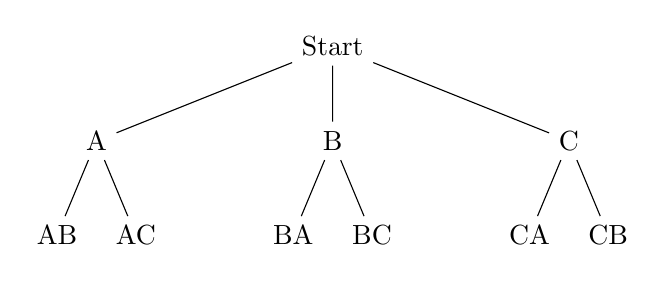
\begin{tikzpicture}[level distance=1.2cm, sibling distance=2cm,
  level 1/.style={sibling distance=3cm},
  level 2/.style={sibling distance=1cm}]
\node {Start}
  child {node {A}
    child {node {AB}}
    child {node {AC}}
  }
  child {node {B}
    child {node {BA}}
    child {node {BC}}
  }
  child {node {C}
    child {node {CA}}
    child {node {CB}}
  };
\end{tikzpicture}
\end{center}
First letter: 3 choices. Second letter: 2 choices (can't repeat). Total: $3 \times 2 = 6$ strings.
\end{example}

\begin{keyresult}
Possibility trees are most useful when:
\begin{itemize}
  \item The number of outcomes is small enough to draw
  \item Choices at each step depend on previous choices
  \item You need to verify your counting is correct
\end{itemize}
For larger problems, use the multiplication/addition rules directly.
\end{keyresult}

\begin{definition}[With vs. without replacement]
\begin{itemize}
  \item \textbf{With replacement:} After selecting an object, it goes back into the pool. Selections are independent.
  \item \textbf{Without replacement:} Once selected, an object is removed from the pool. Later selections have fewer choices.
\end{itemize}
\end{definition}

\begin{proposition}[Counting sequences]
From a set of $n$ distinct elements:
\begin{itemize}
  \item Sequences of length $k$ \textbf{with replacement}: $n^k$
  \item Sequences of length $k$ \textbf{without replacement}: $P(n,k) = \frac{n!}{(n-k)!}$
\end{itemize}
\end{proposition}

\subsection*{Worked examples}

\begin{example}
A license plate consists of 3 letters followed by 3 digits. How many license plates are possible?

\emph{Solution.} Using the multiplication rule:
\begin{itemize}
  \item 3 letters: $26 \times 26 \times 26 = 26^3$ choices (with replacement)
  \item 3 digits: $10 \times 10 \times 10 = 10^3$ choices
\end{itemize}
Total: $26^3 \times 10^3 = 17,576 \times 1000 = 17,576,000$.
\end{example}

\begin{example}
How many 3-letter strings over $\{A, B, C, D\}$ have no repeated letters?

\emph{Solution.} This is a 3-permutation of 4 objects:
\[
P(4, 3) = 4 \times 3 \times 2 = 24
\]
Alternatively: First letter: 4 choices. Second letter: 3 choices (can't repeat first). Third letter: 2 choices.
\end{example}

\begin{example}
A fair die is rolled twice. What is the probability that the sum is 7?

\emph{Solution.}
\begin{itemize}
  \item Sample space: All pairs $(a, b)$ with $a, b \in \{1, 2, 3, 4, 5, 6\}$. Size: $6 \times 6 = 36$.
  \item Event $E$: pairs summing to 7. These are $(1,6), (2,5), (3,4), (4,3), (5,2), (6,1)$. Size: 6.
\end{itemize}
\[
P(E) = \frac{6}{36} = \frac{1}{6}
\]
\end{example}

\begin{example}
How many 5-bit binary strings contain at least one 1?

\emph{Solution (complement counting).}
\begin{itemize}
  \item Total 5-bit strings: $2^5 = 32$
  \item Strings with no 1s: just $00000$, so 1
\end{itemize}
Strings with at least one 1: $32 - 1 = 31$.
\end{example}

\begin{example}
How many integers in $\{1, 2, \ldots, 100\}$ are divisible by 2 or 3?

\emph{Solution (inclusion-exclusion).}
Let $A = \{n : 2 \mid n\}$ and $B = \{n : 3 \mid n\}$.
\begin{itemize}
  \item $|A| = \lfloor 100/2 \rfloor = 50$
  \item $|B| = \lfloor 100/3 \rfloor = 33$
  \item $|A \cap B| = |\{n : 6 \mid n\}| = \lfloor 100/6 \rfloor = 16$
\end{itemize}
\[
|A \cup B| = 50 + 33 - 16 = 67
\]
\end{example}

\begin{example}
Prove: Among any 13 people, at least two share a birth month.

\emph{Solution.} There are 12 months (boxes) and 13 people (objects). By the pigeonhole principle, at least one month contains at least 2 people.
\end{example}

\begin{example}
Prove: In any set of 6 integers, there exist two with the same remainder when divided by 5.

\emph{Solution.} Remainders modulo 5 are in $\{0, 1, 2, 3, 4\}$ (5 boxes). With 6 integers (objects), by pigeonhole, at least two have the same remainder.
\end{example}

\begin{example}
How many ways can 8 people sit in a row if two specific people (Alice and Bob) must sit together?

\emph{Solution.} Treat Alice and Bob as a single ``super-person.'' Then we arrange 7 objects in a row: $7!$ ways. But Alice and Bob can be in either order within their block: 2 ways.

Total: $7! \times 2 = 5040 \times 2 = 10080$.
\end{example}

\begin{example}
How many ways can 8 people sit in a row if Alice and Bob must NOT sit together?

\emph{Solution (complement counting).}
\begin{itemize}
  \item Total arrangements: $8! = 40320$
  \item Arrangements where they sit together: $10080$ (from previous example)
\end{itemize}
Answer: $40320 - 10080 = 30240$.
\end{example}

\begin{example}
A committee of 5 is to be chosen from 8 candidates. In how many ways can this be done if the order of selection matters?

\emph{Solution.} This is a 5-permutation of 8:
\[
P(8, 5) = 8 \times 7 \times 6 \times 5 \times 4 = 6720
\]
\end{example}

\begin{example}
Prove: Among any 5 points placed inside a unit square, at least two are within distance $\frac{\sqrt{2}}{2}$ of each other.

\emph{Solution.} Divide the unit square into 4 smaller squares of side $\frac{1}{2}$. By pigeonhole, at least two of the 5 points lie in the same small square. The maximum distance between two points in a square of side $\frac{1}{2}$ is the diagonal length: $\frac{\sqrt{2}}{2}$.
\end{example}

\begin{commonmistake}
\textbf{Overcounting.} When counting arrangements, make sure you're not counting the same configuration multiple times. Ask yourself:
\begin{itemize}
  \item Does order matter? (permutation vs. combination)
  \item Are objects distinguishable?
  \item Are positions/boxes distinguishable?
\end{itemize}
\end{commonmistake}

\begin{commonmistake}
\textbf{Misapplying the multiplication rule.} The multiplication rule requires that the number of choices at each step is \emph{independent} of previous choices (or carefully accounted for). If earlier choices affect later options, you must account for this.
\end{commonmistake}

\begin{goingdeeper}[Going Deeper: The Algebra of Types]
The counting rules we've learned---multiplication and addition---have a surprising connection to types in programming. This connection reveals why these rules are so fundamental.
For more detail, see the Category Theory Companion, Weeks 4--5.

\subsubsection*{Types Have Sizes}

In programming, a \emph{type} is a set of values. We can count how many values a type has:
\begin{center}
\begin{tabular}{lcc}
\textbf{Type} & \textbf{Description} & \textbf{Size} \\
\hline
\texttt{Void} & empty type (no values) & 0 \\
\texttt{Unit} or \texttt{()} & type with one value & 1 \\
\texttt{Bool} & \texttt{True} or \texttt{False} & 2 \\
\texttt{Char} & ASCII characters & 128 (or 256)
\end{tabular}
\end{center}

\subsubsection*{Products and Sums of Types}

Now here's the magic. If we combine types:
\begin{itemize}
  \item \textbf{Product type} $(A, B)$ (pairs): $|A \times B| = |A| \times |B|$
  \item \textbf{Sum type} \texttt{Either A B}: $|A + B| = |A| + |B|$
\end{itemize}

This is exactly the multiplication and addition rules for counting!

\textbf{Example.} The type \texttt{(Bool, Bool)} has $2 \times 2 = 4$ values:
\[
\texttt{(True, True), (True, False), (False, True), (False, False)}
\]

\textbf{Example.} The type \texttt{Either Bool ()} has $2 + 1 = 3$ values:
\[
\texttt{Left True, Left False, Right ()}
\]

\subsubsection*{Function Types as Exponentials (Map Objects)}
Function types correspond to \textbf{exponentials} in category theory. In $\Set$, the object $B^A$ is the set of all functions $A \to B$. It comes with an \emph{evaluation} map:
\[
\mathrm{ev}: B^A \times A \to B, \quad \mathrm{ev}(f, a) = f(a)
\]
The universal property says: any $g: X \times A \to B$ uniquely corresponds to a map $\tilde{g}: X \to B^A$ (``currying'').

\subsubsection*{Why the Names ``Product'' and ``Sum''?}

This isn't a coincidence! The names come from the fact that type sizes multiply and add. The categorical perspective (from Week 2) explains why:
\begin{itemize}
  \item Products satisfy the universal property of products
  \item Sums (coproducts) satisfy the dual universal property
\end{itemize}

\subsubsection*{Algebraic Laws}

These type operations satisfy the same laws as arithmetic:
\begin{itemize}
  \item $A \times 1 \cong A$ (pairing with unit adds no information)
  \item $A + 0 \cong A$ (sum with empty type is just $A$)
  \item $A \times (B + C) \cong (A \times B) + (A \times C)$ (distributivity)
  \item $A \times B \cong B \times A$ (commutativity)
\end{itemize}

\subsubsection*{Exercises: Types and Counting}

\begin{enumerate}
  \item How many values does the type \texttt{(Bool, Bool, Bool)} have? List them.

  \item How many values does \texttt{Either Bool Bool} have? How is this different from \texttt{(Bool, Bool)}?

  \item If type $A$ has 3 values and type $B$ has 4 values, how many values does $A \times B$ have? How many does $A + B$ have?

  \item The type \texttt{Maybe A} is defined as \texttt{Either () A} (either ``nothing'' or a value of type $A$). If $|A| = n$, what is $|\texttt{Maybe } A|$?

  \item Verify the distributive law by counting: if $|A| = 2$, $|B| = 3$, $|C| = 1$, check that $|A \times (B + C)| = |A \times B| + |A \times C|$.

  \item \textbf{Challenge:} Function types $A \to B$ have $|B|^{|A|}$ values (every function is a choice of output for each input). Verify this for $A = \texttt{Bool}$ and $B = \{1, 2, 3\}$ by listing all functions.
\end{enumerate}
\end{goingdeeper}

\subsection*{Practice}
\begin{enumerate}
  \item A fair die is rolled twice. What is the probability the sum is 7?

  \item How many 5-bit binary strings contain at least one 1?

  \item Use inclusion--exclusion to count integers in $\{1, \ldots, 100\}$ divisible by 2 or 3.

  \item Use the pigeonhole principle to show that among 13 people, two share a birth month.

  \item How many 4-digit PINs (using digits 0--9) have no repeated digits?

  \item A standard deck has 52 cards. How many 5-card hands are possible? (Order doesn't matter---use $\binom{52}{5}$ from Week 5, or just set up the problem.)

  \item How many ways can 6 different books be arranged on a shelf if two specific books must be at the ends?

  \item How many bit strings of length 8 start with 1 or end with 00?

  \item Prove: Among any 10 integers, there exist two whose difference is divisible by 9.

  \item A restaurant offers 3 appetizers, 5 main courses, and 2 desserts. How many different 3-course meals are possible?

  \item How many permutations of ABCDEF contain ABC as a consecutive substring?

  \item Prove: If 5 points are selected from the integer lattice points in $\{0,1,2\}^2$, then two of them have midpoint that is also a lattice point.

  \item Use inclusion-exclusion to count integers in $\{1, \ldots, 1000\}$ divisible by 2, 3, or 5.

  \item Compute $D_5$ (the number of derangements of 5 elements).

  \item Five friends exchange gifts so that no one receives their own gift. How many ways can this be done?

  \item How many permutations of $\{1, 2, 3, 4, 5, 6\}$ have at least one fixed point? (Hint: Use complement counting with derangements.)

  \item Use inclusion-exclusion to count the number of surjective functions from a 4-element set to a 3-element set. (Hint: Let $A_i$ be functions missing element $i$ in the image.)

  \item Two fair dice are rolled. Let $A$ be the event ``the sum is even'' and $B$ be the event ``the sum is at least 10.'' Compute $P(A \mid B)$ and determine whether $A$ and $B$ are independent.

  \item A box contains 3 fair coins and 1 double-headed coin. A coin is chosen uniformly at random and flipped once. If it lands heads, what is the probability the chosen coin was double-headed?

  \item A test for a disease has sensitivity 0.95 and false positive rate 0.02. If 1\% of the population has the disease, compute the probability that a person who tests positive actually has the disease.

  \item Suppose $P(A)=0.4$, $P(B)=0.5$, and $P(A \cap B)=0.2$. Compute $P(A \mid B)$ and $P(A \cup B)$, and determine whether $A$ and $B$ are independent.
\end{enumerate}

\newpage
\section{Week 5: Counting and Probability II}
\subsection*{Reading}
Epp \S 9.5--9.7.

\subsection*{Learning objectives}
\begin{itemize}
  \item Compute combinations and binomial coefficients.
  \item Count with repetition using stars and bars.
  \item Use Pascal's identity and the binomial theorem.
  \item Apply counting techniques to probability problems.
\end{itemize}

\subsection*{Key definitions and facts}
\begin{definition}[Binomial coefficient]
$\binom{n}{k}=\dfrac{n!}{k!(n-k)!}$ counts $k$-element subsets of an $n$-element set.
Equivalently, it is the number of ways to choose $k$ items from $n$ items without regard to order.
\end{definition}

\begin{theorem}[Pascal's identity]
For $1 \leq k \leq n$:
\[
\binom{n}{k} = \binom{n-1}{k-1} + \binom{n-1}{k}
\]
\emph{Combinatorial proof:} Consider element $n$. Either it's in the subset (choose $k-1$ more from $n-1$) or it's not (choose $k$ from $n-1$).
\end{theorem}

\begin{theorem}[Binomial theorem]
$(x+y)^n=\sum_{k=0}^n \binom{n}{k}x^{n-k}y^k$.
\end{theorem}

\begin{theorem}[Stars and bars]
The number of ways to place $n$ identical objects into $k$ distinct bins is $\binom{n+k-1}{k-1}$.
Equivalently, this counts non-negative integer solutions to $x_1 + x_2 + \cdots + x_k = n$.
\end{theorem}

\begin{theorem}[Useful identities]
\begin{itemize}
  \item $\binom{n}{k} = \binom{n}{n-k}$ (symmetry)
  \item $\sum_{k=0}^{n} \binom{n}{k} = 2^n$ (total subsets)
  \item $\sum_{k=0}^{n} (-1)^k \binom{n}{k} = 0$ (alternating sum)
  \item $\binom{n}{0} + \binom{n}{2} + \cdots = \binom{n}{1} + \binom{n}{3} + \cdots = 2^{n-1}$
\end{itemize}
\end{theorem}

\begin{definition}[Multinomial coefficient]
The number of ways to partition $n$ objects into groups of sizes $k_1, k_2, \ldots, k_r$ (where $k_1 + \cdots + k_r = n$) is:
\[
\binom{n}{k_1, k_2, \ldots, k_r} = \frac{n!}{k_1! k_2! \cdots k_r!}
\]
\end{definition}

\subsection*{Worked examples}
\begin{example}
How many solutions are there to $x_1+x_2+x_3=7$ with $x_i\ge 0$?

\emph{Solution.} Using stars and bars: we have 7 stars and need 2 bars to separate into 3 groups.
Total positions: $7 + 2 = 9$. Choose 2 positions for bars: $\binom{9}{2} = \frac{9 \cdot 8}{2} = 36$.
\end{example}

\begin{example}
Prove $\sum_{k=0}^{n} \binom{n}{k} = 2^n$.

\emph{Proof 1 (Binomial theorem):} Set $x = y = 1$ in $(x+y)^n = \sum_{k=0}^n \binom{n}{k}x^{n-k}y^k$.

\emph{Proof 2 (Combinatorial):} LHS counts all subsets of an $n$-element set (choose 0, or 1, or 2, ..., or $n$ elements). RHS: each element is either in or out, giving $2^n$ choices. \qed
\end{example}

\begin{example}
How many ways can the letters of MISSISSIPPI be arranged?

\emph{Solution.} Total 11 letters: M(1), I(4), S(4), P(2).
Using the multinomial coefficient: $\binom{11}{1,4,4,2} = \frac{11!}{1! \cdot 4! \cdot 4! \cdot 2!} = \frac{39916800}{1 \cdot 24 \cdot 24 \cdot 2} = 34650$.
\end{example}

\begin{example}
Prove Pascal's identity: $\binom{n}{k} = \binom{n-1}{k-1} + \binom{n-1}{k}$.

\emph{Algebraic proof:}
\begin{align*}
\binom{n-1}{k-1} + \binom{n-1}{k} &= \frac{(n-1)!}{(k-1)!(n-k)!} + \frac{(n-1)!}{k!(n-k-1)!} \\
&= \frac{(n-1)! \cdot k + (n-1)! \cdot (n-k)}{k!(n-k)!} \\
&= \frac{(n-1)! \cdot n}{k!(n-k)!} = \frac{n!}{k!(n-k)!} = \binom{n}{k}
\end{align*}
\end{example}

\begin{example}
Use the binomial theorem to expand $(2x - 1)^4$.

\emph{Solution.} By the binomial theorem with $a = 2x$ and $b = -1$:
\begin{align*}
(2x - 1)^4 &= \sum_{k=0}^{4} \binom{4}{k} (2x)^{4-k} (-1)^k \\
&= \binom{4}{0}(2x)^4 - \binom{4}{1}(2x)^3 + \binom{4}{2}(2x)^2 - \binom{4}{3}(2x) + \binom{4}{4} \\
&= 1 \cdot 16x^4 - 4 \cdot 8x^3 + 6 \cdot 4x^2 - 4 \cdot 2x + 1 \\
&= 16x^4 - 32x^3 + 24x^2 - 8x + 1
\end{align*}
\end{example}

\begin{example}
How many positive integer solutions are there to $x_1 + x_2 + x_3 = 10$?

\emph{Solution.} Since we want \emph{positive} integers ($x_i \geq 1$), substitute $y_i = x_i - 1$ so $y_i \geq 0$. Then:
\[
(y_1 + 1) + (y_2 + 1) + (y_3 + 1) = 10 \implies y_1 + y_2 + y_3 = 7
\]
Now we count non-negative integer solutions using stars and bars. We have 7 stars and need 2 bars to separate into 3 groups:
\[
\binom{7 + 3 - 1}{3 - 1} = \binom{9}{2} = \frac{9 \cdot 8}{2} = 36
\]
\end{example}

\begin{example}
A committee of 5 is chosen from 6 men and 4 women. How many committees have at least 2 women?

\emph{Solution.} ``At least 2 women'' means 2, 3, or 4 women. Count each case:
\begin{itemize}
  \item 2 women, 3 men: $\binom{4}{2} \binom{6}{3} = 6 \cdot 20 = 120$
  \item 3 women, 2 men: $\binom{4}{3} \binom{6}{2} = 4 \cdot 15 = 60$
  \item 4 women, 1 man: $\binom{4}{4} \binom{6}{1} = 1 \cdot 6 = 6$
\end{itemize}
Total: $120 + 60 + 6 = 186$.

\emph{Alternative (complement):} Total committees: $\binom{10}{5} = 252$. Committees with fewer than 2 women:
\begin{itemize}
  \item 0 women: $\binom{4}{0}\binom{6}{5} = 6$
  \item 1 woman: $\binom{4}{1}\binom{6}{4} = 4 \cdot 15 = 60$
\end{itemize}
Answer: $252 - 6 - 60 = 186$. \checkmark
\end{example}

\begin{example}
In how many ways can 10 identical apples be distributed among 4 children?

\emph{Solution.} This is distributing $n = 10$ identical objects into $k = 4$ distinct bins. By stars and bars:
\[
\binom{10 + 4 - 1}{4 - 1} = \binom{13}{3} = \frac{13 \cdot 12 \cdot 11}{3 \cdot 2 \cdot 1} = \frac{1716}{6} = 286
\]
\end{example}

\begin{example}
Prove combinatorially: $\binom{n}{0} + \binom{n}{1} + \binom{n}{2} + \cdots + \binom{n}{n} = 2^n$.

\emph{Proof.} The LHS counts subsets of an $n$-element set by size: there are $\binom{n}{k}$ subsets of size $k$.

The RHS counts subsets directly: each of the $n$ elements is either in or out of the subset, giving $2^n$ choices.

Both count the same thing (total number of subsets), so they're equal. \qed
\end{example}

\subsection*{Practice}
\begin{enumerate}
  \item Compute $\binom{12}{5}$.
  \item How many 8-card poker hands contain exactly 3 hearts?
  \item Prove Pascal's identity: $\binom{n}{k}=\binom{n-1}{k}+\binom{n-1}{k-1}$.
  \item Use the binomial theorem to expand $(2x-1)^5$.
  \item How many positive integer solutions are there to $x_1 + x_2 + x_3 + x_4 = 15$?
  \item Prove: $\binom{n}{0}^2 + \binom{n}{1}^2 + \cdots + \binom{n}{n}^2 = \binom{2n}{n}$.
  \item A committee of 5 is to be chosen from 6 men and 4 women. How many committees have at least 2 women?
\end{enumerate}

\newpage
\section{Week 6: Expected Value and Introduction to Graphs}
\subsection*{Reading}
Epp \S 9.8; 10.1; 10.2.

\subsection*{Learning objectives}
\begin{itemize}
  \item Define and compute expected value for discrete random variables.
  \item Apply linearity of expectation to simplify calculations.
  \item Use indicator random variables for counting.
  \item Define graphs, vertices, edges, and basic terminology.
  \item Apply the handshake theorem to relate degrees and edges.
  \item Distinguish simple graphs, multigraphs, and digraphs.
\end{itemize}

\subsection*{Part I: Expected Value}

\begin{definition}[Probability axioms (Kolmogorov)]
A \textbf{probability measure} on a sample space $S$ is a function $P$ assigning to each event $A \subseteq S$ a number $P(A)$ satisfying:
\begin{enumerate}
  \item \textbf{Non-negativity:} $P(A) \geq 0$ for all events $A$.
  \item \textbf{Normalization:} $P(S) = 1$.
  \item \textbf{Additivity:} If $A_1, A_2, \ldots$ are pairwise disjoint events, then
  \[
  P\left(\bigcup_{i=1}^{\infty} A_i\right) = \sum_{i=1}^{\infty} P(A_i)
  \]
\end{enumerate}
\end{definition}

\begin{proposition}[Consequences of the axioms]
From the three axioms, we can derive:
\begin{itemize}
  \item $P(\emptyset) = 0$
  \item $P(A^c) = 1 - P(A)$
  \item If $A \subseteq B$, then $P(A) \leq P(B)$
  \item $P(A \cup B) = P(A) + P(B) - P(A \cap B)$
  \item $0 \leq P(A) \leq 1$ for all events $A$
\end{itemize}
\end{proposition}

\begin{definition}[Random variable]
A \textbf{random variable} $X$ on a sample space $S$ is a function $X: S \to \R$ that assigns a real number to each outcome. For discrete random variables, the possible values form a finite or countably infinite set.
\end{definition}

\begin{definition}[Expected value]
The \textbf{expected value} (or \textbf{expectation} or \textbf{mean}) of a discrete random variable $X$ with possible values $x_1, x_2, \ldots$ and probabilities $p_i = P(X = x_i)$ is:
\[
E[X] = \sum_i x_i \cdot P(X = x_i) = \sum_i x_i \cdot p_i
\]
provided the sum converges absolutely.
\end{definition}

\begin{theorem}[Linearity of expectation]
For any random variables $X$ and $Y$ (even if dependent) and constants $a, b \in \R$:
\[
E[aX + bY] = aE[X] + bE[Y]
\]
More generally, for any $X_1, \ldots, X_n$:
\[
E\left[\sum_{i=1}^n X_i\right] = \sum_{i=1}^n E[X_i]
\]
\end{theorem}

\begin{keyresult}
Linearity of expectation is extremely powerful because it works \emph{regardless of whether the random variables are independent}. This makes many expected value calculations surprisingly simple.
\end{keyresult}

\begin{definition}[Indicator random variable]
An \textbf{indicator random variable} $I_A$ for event $A$ is:
\[
I_A = \begin{cases} 1 & \text{if } A \text{ occurs} \\ 0 & \text{otherwise} \end{cases}
\]
Note that $E[I_A] = P(A)$.
\end{definition}

\begin{theorem}[Counting with indicators]
If $X$ counts the number of events $A_1, \ldots, A_n$ that occur, then:
\[
X = I_{A_1} + I_{A_2} + \cdots + I_{A_n}
\]
and by linearity:
\[
E[X] = P(A_1) + P(A_2) + \cdots + P(A_n)
\]
\end{theorem}

\begin{definition}[Common distributions]
\begin{itemize}
  \item \textbf{Bernoulli($p$):} $X = 1$ with probability $p$, $X = 0$ with probability $1-p$. $E[X] = p$.

  \item \textbf{Binomial($n, p$):} Number of successes in $n$ independent trials, each with success probability $p$. $E[X] = np$.

  \item \textbf{Geometric($p$):} Number of trials until first success. $E[X] = 1/p$.

  \item \textbf{Uniform on $\{1, \ldots, n\}$:} Each value equally likely. $E[X] = (n+1)/2$.
\end{itemize}
\end{definition}

\begin{definition}[Variance and standard deviation]
The \textbf{variance} of $X$ is:
\[
\text{Var}(X) = E[(X - E[X])^2] = E[X^2] - (E[X])^2
\]
The \textbf{standard deviation} is $\sigma = \sqrt{\text{Var}(X)}$.
\end{definition}

\subsection*{Part II: Introduction to Graphs}

\begin{definition}[Graph]
A \textbf{graph} $G = (V, E)$ consists of:
\begin{itemize}
  \item $V$: a finite nonempty set of \textbf{vertices} (or nodes)
  \item $E$: a set of \textbf{edges}, each connecting two vertices
\end{itemize}
\end{definition}

\begin{definition}[Types of graphs]
\begin{itemize}
  \item \textbf{Simple graph:} No loops (edges from a vertex to itself) and no multiple edges between the same pair of vertices.
  \item \textbf{Multigraph:} Allows multiple edges between the same pair of vertices.
  \item \textbf{Pseudograph:} Allows loops and multiple edges.
  \item \textbf{Directed graph (digraph):} Edges have direction, going from one vertex to another.
\end{itemize}
\end{definition}

\begin{definition}[Basic terminology]
Let $G = (V, E)$ be a graph.
\begin{itemize}
  \item Two vertices are \textbf{adjacent} if an edge connects them.
  \item An edge is \textbf{incident} to its endpoints.
  \item The \textbf{degree} $\deg(v)$ of vertex $v$ is the number of edges incident to $v$ (loops count twice).
  \item A vertex with degree 0 is \textbf{isolated}.
  \item A vertex with degree 1 is a \textbf{leaf} (or pendant vertex).
  \item The \textbf{neighborhood} $N(v)$ is the set of vertices adjacent to $v$.
\end{itemize}
\end{definition}

\begin{theorem}[Handshake theorem]
In any graph $G = (V, E)$:
\[
\sum_{v \in V} \deg(v) = 2|E|
\]
\emph{Proof idea:} Each edge contributes exactly 2 to the sum of degrees (1 to each endpoint). \qed
\end{theorem}

\begin{corollary}
In any graph, the number of vertices with odd degree is even.
\end{corollary}

\begin{definition}[Special graphs]
\begin{itemize}
  \item \textbf{Complete graph $K_n$:} Simple graph on $n$ vertices with all possible edges. Has $\binom{n}{2} = \frac{n(n-1)}{2}$ edges.

  \item \textbf{Cycle $C_n$:} Graph on $n$ vertices forming a single cycle. Has $n$ edges.

  \item \textbf{Path $P_n$:} Graph on $n$ vertices forming a single path. Has $n-1$ edges.

  \item \textbf{Complete bipartite graph $K_{m,n}$:} Vertices partitioned into sets of sizes $m$ and $n$; every vertex in one set is adjacent to every vertex in the other. Has $mn$ edges.

  \item \textbf{$n$-cube $Q_n$:} Vertices are $n$-bit strings; edges connect strings differing in exactly one bit. Has $2^n$ vertices and $n \cdot 2^{n-1}$ edges.
\end{itemize}
\end{definition}

\begin{definition}[Degree sequence]
The \textbf{degree sequence} of a graph is the list of vertex degrees in non-increasing order. For example, $K_4$ has degree sequence $(3, 3, 3, 3)$.
\end{definition}

\begin{theorem}[Degree sequence realizability]
A sequence of non-negative integers $(d_1, d_2, \ldots, d_n)$ with $d_1 \geq d_2 \geq \cdots \geq d_n$ is the degree sequence of a simple graph if and only if:
\begin{enumerate}
  \item The sum $\sum d_i$ is even.
  \item The sequence satisfies the Erdős--Gallai conditions (or can be checked using the Havel--Hakimi algorithm).
\end{enumerate}
\end{theorem}

\begin{definition}[Subgraph]
$H = (V', E')$ is a \textbf{subgraph} of $G = (V, E)$ if $V' \subseteq V$ and $E' \subseteq E$.

$H$ is an \textbf{induced subgraph} if $E'$ contains all edges of $G$ whose endpoints are both in $V'$.
\end{definition}

\begin{definition}[Graph complement]
The \textbf{complement} $\overline{G}$ of a simple graph $G = (V, E)$ has the same vertices as $G$, and two vertices are adjacent in $\overline{G}$ iff they are not adjacent in $G$.
\end{definition}

\subsection*{Worked examples}

\begin{example}
A fair die is rolled. Let $X$ be the outcome. Compute $E[X]$.

\emph{Solution.} Each outcome $1, 2, 3, 4, 5, 6$ has probability $\frac{1}{6}$.
\[
E[X] = 1 \cdot \frac{1}{6} + 2 \cdot \frac{1}{6} + 3 \cdot \frac{1}{6} + 4 \cdot \frac{1}{6} + 5 \cdot \frac{1}{6} + 6 \cdot \frac{1}{6} = \frac{21}{6} = 3.5
\]
\end{example}

\begin{example}
A coin is flipped 10 times. What is the expected number of heads?

\emph{Solution.} Let $X_i = 1$ if flip $i$ is heads, 0 otherwise. Then $X = X_1 + \cdots + X_{10}$ counts heads.

By linearity: $E[X] = E[X_1] + \cdots + E[X_{10}] = 10 \cdot \frac{1}{2} = 5$.
\end{example}

\begin{example}
In a random permutation of $n$ elements, what is the expected number of fixed points (elements in their original position)?

\emph{Solution.} Let $X_i = 1$ if element $i$ is in position $i$. Then $X = \sum_{i=1}^n X_i$ counts fixed points.

$P(\text{element } i \text{ is in position } i) = \frac{1}{n}$ (any of the $n!$ permutations, the element has $\frac{(n-1)!}{n!} = \frac{1}{n}$ chance of being fixed).

By linearity: $E[X] = n \cdot \frac{1}{n} = 1$.

Remarkably, the expected number of fixed points is exactly 1, regardless of $n$!
\end{example}

\begin{example}
What is the expected number of times we must roll a die to get a 6?

\emph{Solution.} This is a geometric random variable with success probability $p = \frac{1}{6}$.

$E[X] = \frac{1}{p} = 6$.
\end{example}

\begin{example}
Verify the handshake theorem for $K_4$.

\emph{Solution.} $K_4$ has 4 vertices, each with degree 3 (connected to all others).
\begin{itemize}
  \item Sum of degrees: $3 + 3 + 3 + 3 = 12$
  \item Number of edges: $\binom{4}{2} = 6$
  \item Check: $2 \times 6 = 12$ \checkmark
\end{itemize}
\end{example}

\begin{example}
Is there a simple graph with degree sequence $(3, 3, 2, 2, 2)$?

\emph{Solution.} Sum of degrees: $3 + 3 + 2 + 2 + 2 = 12$, which is even. \checkmark

Using Havel--Hakimi: Sort: $(3, 3, 2, 2, 2)$. Remove 3 and subtract 1 from next 3 degrees: $(2, 1, 1, 2)$. Sort: $(2, 2, 1, 1)$. Remove 2: $(1, 0, 1)$. Sort: $(1, 1, 0)$. Remove 1: $(0, 0)$. This is realizable (empty graph).

Yes, such a graph exists.
\end{example}

\begin{example}
How many edges does the $n$-cube $Q_n$ have?

\emph{Solution.} $Q_n$ has $2^n$ vertices, each an $n$-bit string. Each vertex has degree $n$ (can flip any of $n$ bits).

Sum of degrees: $n \cdot 2^n$.

By handshake theorem: $|E| = \frac{n \cdot 2^n}{2} = n \cdot 2^{n-1}$.
\end{example}

\begin{example}
Prove: The sum of degrees in a tree on $n$ vertices is $2(n-1)$.

\emph{Solution.} A tree on $n$ vertices has exactly $n-1$ edges (this is a standard fact---see Week 8). By the handshake theorem:
\[
\sum_{v \in V} \deg(v) = 2|E| = 2(n-1)
\]
\end{example}

\begin{example}
Show that every simple graph on $n \geq 2$ vertices has at least two vertices of the same degree.

\emph{Solution.} Degrees in a simple graph range from 0 to $n-1$. That's $n$ possible values. But if some vertex has degree 0 (isolated), no vertex can have degree $n-1$ (connected to all). So at most $n-1$ distinct degrees are possible among $n$ vertices. By pigeonhole, two must share a degree.
\end{example}

\begin{commonmistake}
\textbf{Forgetting linearity works for dependent variables.} The formula $E[X + Y] = E[X] + E[Y]$ does NOT require $X$ and $Y$ to be independent. Many students add independence as an assumption when it's unnecessary.
\end{commonmistake}

\begin{commonmistake}
\textbf{Confusing $E[X \cdot Y]$ with $E[X] \cdot E[Y]$.} These are equal only when $X$ and $Y$ are independent. In general, $E[XY] = E[X]E[Y] + \text{Cov}(X,Y)$.
\end{commonmistake}

\subsection*{Practice}
\begin{enumerate}
  \item A coin is flipped 10 times. What is the expected number of heads?

  \item Show that the sum of degrees in a tree on $n$ vertices is $2(n-1)$.

  \item Find $E[X]$ for a geometric random variable with success probability $p$.

  \item Decide whether a graph with degree sequence $(3, 3, 2, 2, 2)$ is possible.

  \item In a random permutation of $\{1, 2, \ldots, n\}$, what is the expected number of elements greater than all previous elements?

  \item How many edges does $K_{4,5}$ have? What are the degrees of the vertices?

  \item Prove that the complement of $K_n$ is an empty graph (no edges).

  \item A bag contains 5 red and 3 blue marbles. Two are drawn without replacement. What is the expected number of red marbles drawn?

  \item Show that the number of edges in a simple graph on $n$ vertices is at most $\binom{n}{2}$.

  \item Using the handshake theorem, prove: If $G$ is a graph where every vertex has degree at least $k$, then $|E| \geq \frac{k|V|}{2}$.

  \item Prove that every graph has an even number of vertices with odd degree.

  \item In a room of 100 people, everyone shakes hands with exactly 3 other people. Is this possible?
\end{enumerate}

\newpage
\section{Week 7: Graph Theory I --- Paths and Connectivity}
\subsection*{Reading}
Epp \S 10.1--10.3.

\subsection*{Learning objectives}
\begin{itemize}
  \item Distinguish walks, trails, paths, and circuits.
  \item Apply Euler's criteria for trails and circuits.
  \item Determine graph connectivity and connected components.
  \item Represent graphs with adjacency matrices and adjacency lists.
  \item Determine whether two graphs are isomorphic.
\end{itemize}

\subsection*{Key definitions and facts}

\begin{definition}[Walk]
A \textbf{walk} in a graph $G$ from vertex $v_0$ to vertex $v_n$ is a sequence:
\[
v_0, e_1, v_1, e_2, v_2, \ldots, e_n, v_n
\]
where each $e_i$ is an edge connecting $v_{i-1}$ and $v_i$. The \textbf{length} of the walk is $n$ (the number of edges).
\end{definition}

\begin{definition}[Types of walks]
\begin{itemize}
  \item A \textbf{trail} is a walk with no repeated edges.
  \item A \textbf{path} is a walk with no repeated vertices (hence no repeated edges).
  \item A \textbf{closed walk} is a walk where $v_0 = v_n$.
  \item A \textbf{circuit} (or closed trail) is a closed walk with no repeated edges.
  \item A \textbf{cycle} (or simple circuit) is a circuit with no repeated vertices except $v_0 = v_n$.
\end{itemize}
\end{definition}

\begin{proposition}[Path existence]
If there is a walk from $u$ to $v$ in a graph, then there is a path from $u$ to $v$.
\end{proposition}

\begin{definition}[Connectivity]
\begin{itemize}
  \item A graph is \textbf{connected} if there is a path between every pair of vertices.
  \item A \textbf{connected component} of a graph is a maximal connected subgraph.
  \item A \textbf{cut vertex} (or articulation point) is a vertex whose removal disconnects the graph.
  \item A \textbf{bridge} is an edge whose removal disconnects the graph.
\end{itemize}
\end{definition}

\begin{definition}[Euler trail and circuit]
An \textbf{Euler trail} is a trail that uses every edge of the graph exactly once.
An \textbf{Euler circuit} is a circuit that uses every edge exactly once (starts and ends at the same vertex).
\end{definition}

\begin{theorem}[Euler's theorem]
Let $G$ be a connected graph.
\begin{enumerate}
  \item $G$ has an \textbf{Euler circuit} if and only if every vertex has even degree.
  \item $G$ has an \textbf{Euler trail} (but no Euler circuit) if and only if exactly two vertices have odd degree. In this case, the trail must start and end at the odd-degree vertices.
\end{enumerate}
\end{theorem}

\begin{keyresult}
To check if a connected graph has an Euler circuit or trail:
\begin{enumerate}
  \item Count vertices of odd degree.
  \item 0 odd-degree vertices $\Rightarrow$ Euler circuit exists.
  \item 2 odd-degree vertices $\Rightarrow$ Euler trail exists (but no circuit).
  \item $>2$ odd-degree vertices $\Rightarrow$ no Euler trail.
\end{enumerate}
\end{keyresult}

\begin{definition}[Hamiltonian path and cycle]
A \textbf{Hamiltonian path} visits every vertex exactly once.
A \textbf{Hamiltonian cycle} is a cycle that visits every vertex exactly once (except returning to start).
\end{definition}

\begin{remark}
Unlike Euler paths/circuits, there is no simple characterization for when Hamiltonian paths/cycles exist. Determining existence is NP-complete.
\end{remark}

\subsection*{Graph representations}

\begin{definition}[Adjacency matrix]
The \textbf{adjacency matrix} $A$ of a graph $G$ with $n$ vertices is an $n \times n$ matrix where:
\[
A_{ij} = \text{number of edges between vertex } i \text{ and vertex } j
\]
For a simple graph, $A_{ij} \in \{0, 1\}$. The matrix is symmetric for undirected graphs.
\end{definition}

\begin{proposition}[Properties of adjacency matrices]
For the adjacency matrix $A$ of a simple graph:
\begin{itemize}
  \item The sum of row $i$ (or column $i$) equals $\deg(v_i)$.
  \item The sum of all entries equals $2|E|$.
  \item The diagonal is all zeros (no loops).
  \item $(A^k)_{ij}$ counts the number of walks of length $k$ from $v_i$ to $v_j$.
\end{itemize}
\end{proposition}

\begin{definition}[Adjacency list]
An \textbf{adjacency list} representation stores, for each vertex, a list of its neighbors. This is more space-efficient for sparse graphs.
\end{definition}

\subsection*{Graph isomorphism}

\begin{definition}[Graph isomorphism]
Two graphs $G_1 = (V_1, E_1)$ and $G_2 = (V_2, E_2)$ are \textbf{isomorphic}, written $G_1 \cong G_2$, if there exists a bijection $f: V_1 \to V_2$ such that:
\[
\{u, v\} \in E_1 \iff \{f(u), f(v)\} \in E_2
\]
The function $f$ is called an \textbf{isomorphism}.
\end{definition}

\begin{theorem}[Isomorphism invariants]
If $G_1 \cong G_2$, then:
\begin{enumerate}
  \item $|V_1| = |V_2|$
  \item $|E_1| = |E_2|$
  \item They have the same degree sequence
  \item They have the same number of cycles of each length
  \item They have the same number of connected components
  \item Corresponding subgraphs are isomorphic
\end{enumerate}
These are \emph{necessary} but not \emph{sufficient} conditions for isomorphism.
\end{theorem}

\begin{strategy}
To show two graphs are NOT isomorphic, find an invariant they don't share. To show they ARE isomorphic, construct an explicit bijection and verify edge preservation.
\end{strategy}

\begin{definition}[Automorphism]
An \textbf{automorphism} of a graph $G$ is an isomorphism from $G$ to itself. The set of all automorphisms forms a group under composition.
\end{definition}

\subsection*{Distance and diameter}

\begin{definition}[Distance]
The \textbf{distance} $d(u, v)$ between vertices $u$ and $v$ is the length of the shortest path between them. If no path exists, $d(u, v) = \infty$.
\end{definition}

\begin{definition}[Eccentricity, radius, diameter]
\begin{itemize}
  \item The \textbf{eccentricity} of a vertex $v$ is the maximum distance from $v$ to any other vertex: $\max_{u} d(v, u)$.
  \item The \textbf{diameter} of a connected graph is the maximum eccentricity.
  \item The \textbf{radius} is the minimum eccentricity.
  \item A \textbf{center} is a vertex with minimum eccentricity.
\end{itemize}
\end{definition}

\subsection*{Graph coloring}

\begin{definition}[Vertex coloring]
A \textbf{(proper) vertex coloring} of a graph $G$ is an assignment of colors to vertices such that no two adjacent vertices share the same color. A \textbf{$k$-coloring} uses at most $k$ colors.
\end{definition}

\begin{definition}[Chromatic number]
The \textbf{chromatic number} $\chi(G)$ is the minimum number of colors needed to properly color $G$.
\end{definition}

\begin{theorem}[Chromatic number bounds]
For any graph $G$:
\begin{enumerate}
  \item $\chi(G) \geq \omega(G)$, where $\omega(G)$ is the size of the largest clique (complete subgraph).
  \item $\chi(G) \leq \Delta(G) + 1$, where $\Delta(G)$ is the maximum degree.
  \item If $G$ is connected and not a complete graph or odd cycle, then $\chi(G) \leq \Delta(G)$ (Brooks' theorem).
\end{enumerate}
\end{theorem}

\begin{theorem}[Chromatic numbers of special graphs]
\begin{itemize}
  \item $\chi(K_n) = n$ (complete graph needs $n$ colors)
  \item $\chi(C_n) = 2$ if $n$ is even; $\chi(C_n) = 3$ if $n$ is odd
  \item $\chi(K_{m,n}) = 2$ (bipartite graphs are 2-colorable)
  \item A tree with at least one edge has $\chi(T) = 2$
\end{itemize}
\end{theorem}

\begin{definition}[Bipartite graph]
A graph is \textbf{bipartite} if its vertices can be partitioned into two sets such that every edge connects a vertex in one set to a vertex in the other. Equivalently, $G$ is bipartite iff $\chi(G) \leq 2$.
\end{definition}

\begin{theorem}[Bipartite characterization]
A graph is bipartite if and only if it contains no odd-length cycle.
\end{theorem}

\begin{example}
Is the Petersen graph 3-colorable?

\emph{Solution.} The Petersen graph contains triangles (3-cycles), so $\chi \geq 3$. In fact, $\chi(\text{Petersen}) = 3$. You can verify by constructing a 3-coloring: color the outer 5-cycle with alternating colors (using 3 since it's odd), then color the inner 5-cycle consistently.
\end{example}

\subsection*{Planar graphs}

\begin{definition}[Planar graph]
A graph is \textbf{planar} if it can be drawn in the plane with no edges crossing (except at vertices). Such a drawing is called a \textbf{planar embedding}.
\end{definition}

\begin{definition}[Faces]
In a planar embedding, the plane is divided into \textbf{faces} (regions), including one unbounded \textbf{outer face}. The boundary of each face consists of edges and vertices.
\end{definition}

\begin{theorem}[Euler's formula for planar graphs]
For a connected planar graph with $V$ vertices, $E$ edges, and $F$ faces:
\[
V - E + F = 2
\]
\end{theorem}

\begin{example}
Verify Euler's formula for the tetrahedron graph $K_4$.

\emph{Solution.} $K_4$ has $V = 4$ vertices and $E = \binom{4}{2} = 6$ edges. Drawing it as a triangle with a point in the center gives $F = 4$ faces (3 inner triangles + 1 outer face).

Check: $4 - 6 + 4 = 2$. \checkmark
\end{example}

\begin{theorem}[Edge bound for planar graphs]
For a connected planar graph with $V \geq 3$ vertices:
\[
E \leq 3V - 6
\]
If the graph has no triangles (is triangle-free), then $E \leq 2V - 4$.
\end{theorem}

\begin{corollary}
$K_5$ and $K_{3,3}$ are not planar.
\end{corollary}

\begin{proof}
For $K_5$: $V = 5$, $E = 10$. But $3V - 6 = 9 < 10$. Violates the bound.

For $K_{3,3}$: $V = 6$, $E = 9$. Since $K_{3,3}$ is bipartite, it has no triangles, so we need $E \leq 2V - 4 = 8 < 9$. Violates the bound.
\end{proof}

\begin{theorem}[Kuratowski's theorem]
A graph is planar if and only if it contains no subgraph that is a subdivision of $K_5$ or $K_{3,3}$.

(A \textbf{subdivision} is obtained by inserting vertices of degree 2 into edges.)
\end{theorem}

\begin{theorem}[Four Color Theorem]
Every planar graph can be colored with at most 4 colors: $\chi(G) \leq 4$ for planar $G$.
\end{theorem}

\begin{remark}
The Four Color Theorem was proved in 1976 using computer assistance to check thousands of cases. Simpler proofs exist but none are ``hand-checkable.''
\end{remark}

\begin{example}
Show that the cube graph $Q_3$ is planar.

\emph{Solution.} $Q_3$ has $V = 8$ vertices and $E = 12$ edges. Check: $3V - 6 = 18 \geq 12$. \checkmark (This doesn't prove planarity, but it's consistent.)

To prove planarity, we draw $Q_3$ without crossings: draw the outer square as the front face, the inner square as the back face, and connect corresponding vertices.
\end{example}

\begin{strategy}
To show a graph is NOT planar:
\begin{enumerate}
  \item Show it violates $E \leq 3V - 6$, or
  \item Find a $K_5$ or $K_{3,3}$ subdivision.
\end{enumerate}
To show a graph IS planar:
\begin{enumerate}
  \item Draw it without crossings, or
  \item Prove $V$ and $E$ satisfy the bounds (necessary but not sufficient).
\end{enumerate}
\end{strategy}

\subsection*{Worked examples}

\begin{example}
Does a connected graph with degrees $(2, 2, 2, 4, 4)$ have an Euler circuit?

\emph{Solution.} All degrees are even (2, 2, 2, 4, 4), so yes, an Euler circuit exists by Euler's theorem.
\end{example}

\begin{example}
Does the graph $K_4$ (complete graph on 4 vertices) have an Euler circuit?

\emph{Solution.} In $K_4$, each vertex has degree 3 (odd). All 4 vertices have odd degree. Since we need 0 or 2 vertices of odd degree for an Euler trail/circuit, $K_4$ has neither.
\end{example}

\begin{example}
Does the graph $K_5$ have an Euler circuit?

\emph{Solution.} In $K_5$, each vertex has degree 4 (even). All vertices have even degree, so $K_5$ has an Euler circuit.
\end{example}

\begin{example}
Find the adjacency matrix for the cycle $C_4$ on vertices $\{1, 2, 3, 4\}$.

\emph{Solution.} The edges are $\{1,2\}, \{2,3\}, \{3,4\}, \{4,1\}$.
\[
A = \begin{pmatrix}
0 & 1 & 0 & 1 \\
1 & 0 & 1 & 0 \\
0 & 1 & 0 & 1 \\
1 & 0 & 1 & 0
\end{pmatrix}
\]
\end{example}

\begin{example}
Show that the sum of entries in an adjacency matrix of a simple graph equals $2|E|$.

\emph{Solution.} Each edge $\{u, v\}$ contributes 1 to entry $(u, v)$ and 1 to entry $(v, u)$, for a total of 2 per edge. Thus the sum equals $2|E|$.
\end{example}

\begin{example}
Determine whether these two graphs are isomorphic:

$G_1$: vertices $\{a, b, c, d\}$, edges $\{a,b\}, \{b,c\}, \{c,d\}, \{d,a\}$

$G_2$: vertices $\{1, 2, 3, 4\}$, edges $\{1,2\}, \{2,3\}, \{3,4\}, \{4,1\}$

\emph{Solution.} Both are cycles of length 4.
\begin{itemize}
  \item Same number of vertices: 4 \checkmark
  \item Same number of edges: 4 \checkmark
  \item Same degree sequence: $(2, 2, 2, 2)$ \checkmark
\end{itemize}

The bijection $f: a \mapsto 1, b \mapsto 2, c \mapsto 3, d \mapsto 4$ preserves edges:
$\{a,b\} \mapsto \{1,2\}$, $\{b,c\} \mapsto \{2,3\}$, $\{c,d\} \mapsto \{3,4\}$, $\{d,a\} \mapsto \{4,1\}$. All edges match, so $G_1 \cong G_2$.
\end{example}

\begin{example}
Prove that $C_5$ and $K_5$ are not isomorphic.

\emph{Solution.} $C_5$ has 5 edges (a cycle). $K_5$ has $\binom{5}{2} = 10$ edges. Since they have different numbers of edges, they are not isomorphic.
\end{example}

\begin{example}
Are two graphs with the same degree sequence necessarily isomorphic?

\emph{Solution.} No! Consider:
\begin{itemize}
  \item $G_1$: a 6-cycle $C_6$. Degree sequence: $(2, 2, 2, 2, 2, 2)$.
  \item $G_2$: two disjoint triangles $K_3 \sqcup K_3$. Degree sequence: $(2, 2, 2, 2, 2, 2)$.
\end{itemize}
Same degree sequence, but $G_1$ is connected and $G_2$ is not. Not isomorphic.
\end{example}

\begin{example}
Find the diameter of the complete graph $K_n$.

\emph{Solution.} Every pair of vertices is connected by an edge, so $d(u, v) = 1$ for all $u \neq v$. The diameter is 1.
\end{example}

\begin{example}
Find an Euler trail in a graph with vertices $\{A, B, C, D\}$ and edges
\[
\{A,B\}, \{A,C\}, \{B,C\}, \{B,D\}, \{C,D\}.
\]

\emph{Solution.} First, check degrees: $\deg(A) = 2$, $\deg(B) = 3$, $\deg(C) = 3$, $\deg(D) = 2$.

Odd-degree vertices: $B$ and $C$ (exactly 2). So an Euler trail exists, starting and ending at $B$ and $C$.

One Euler trail starting at $B$: $B \to A \to C \to B \to D \to C$.

Verify: Uses edges $\{B,A\}, \{A,C\}, \{C,B\}, \{B,D\}, \{D,C\}$ --- all 5 edges, each exactly once. \checkmark
\end{example}

\begin{example}
Compute $A^2$ for the path graph $P_3$ on vertices $\{1, 2, 3\}$ with edges $\{1,2\}$ and $\{2,3\}$. Interpret the result.

\emph{Solution.}
\[
A = \begin{pmatrix} 0 & 1 & 0 \\ 1 & 0 & 1 \\ 0 & 1 & 0 \end{pmatrix}
\]
\[
A^2 = \begin{pmatrix} 0 & 1 & 0 \\ 1 & 0 & 1 \\ 0 & 1 & 0 \end{pmatrix}
\begin{pmatrix} 0 & 1 & 0 \\ 1 & 0 & 1 \\ 0 & 1 & 0 \end{pmatrix}
= \begin{pmatrix} 1 & 0 & 1 \\ 0 & 2 & 0 \\ 1 & 0 & 1 \end{pmatrix}
\]

Interpretation: $(A^2)_{ij}$ is the number of walks of length 2 from $i$ to $j$.
\begin{itemize}
  \item $(A^2)_{11} = 1$: one walk $1 \to 2 \to 1$.
  \item $(A^2)_{13} = 1$: one walk $1 \to 2 \to 3$.
  \item $(A^2)_{22} = 2$: two walks $2 \to 1 \to 2$ and $2 \to 3 \to 2$.
\end{itemize}
\end{example}

\begin{commonmistake}
\textbf{Confusing Euler and Hamiltonian.}
\begin{itemize}
  \item Euler: visits every \emph{edge} exactly once.
  \item Hamiltonian: visits every \emph{vertex} exactly once.
\end{itemize}
Euler has a simple characterization (degree conditions). Hamiltonian does not.
\end{commonmistake}

\begin{commonmistake}
\textbf{Thinking matching invariants proves isomorphism.} Equal vertex count, edge count, and degree sequence are \emph{necessary} but not \emph{sufficient} for isomorphism. You must construct a bijection or find a distinguishing property.
\end{commonmistake}

\begin{goingdeeper}[Going Deeper: Graphs Generate Categories]
The categorical thread continues: graphs give rise to categories, and this perspective illuminates why adjacency matrices count paths.

\subsubsection*{The Free Category on a Graph}

Given a directed graph $G$, we can build a category $\mathbf{Path}(G)$:
\begin{itemize}
  \item \textbf{Objects:} Vertices of $G$
  \item \textbf{Morphisms from $u$ to $v$:} Directed paths from $u$ to $v$
  \item \textbf{Composition:} Concatenation of paths
  \item \textbf{Identity at $v$:} The empty path (length 0) at $v$
\end{itemize}

This is called the \emph{free category} on $G$---it's the category with ``just enough structure'' to capture the graph.

\textbf{Example.} For the graph $1 \to 2 \to 3$:
\begin{itemize}
  \item Morphisms $1 \to 3$: just the path $1 \to 2 \to 3$ (one morphism)
  \item Morphisms $2 \to 2$: just the empty path $\id_2$ (one morphism)
  \item Morphisms $3 \to 1$: none (no path backwards)
\end{itemize}

\textbf{Example.} For a cycle $1 \to 2 \to 3 \to 1$:
\begin{itemize}
  \item Morphisms $1 \to 1$: empty path, $1 \to 2 \to 3 \to 1$, twice around, thrice around, ...
  \item This is infinite! The cycle generates infinitely many paths.
\end{itemize}

\subsubsection*{Adjacency Matrices Count Morphisms}

Here's the key insight: $(A^k)_{ij}$ counts the number of \textbf{morphisms of length $k$} from $i$ to $j$ in $\mathbf{Path}(G)$.

Why? Let's see for $k = 2$:
\[
(A^2)_{ij} = \sum_m A_{im} \cdot A_{mj}
\]
Each term $A_{im} \cdot A_{mj}$ counts paths that go $i \to m \to j$ (one for each intermediate vertex $m$ with edges from $i$ and to $j$).

This is exactly the \textbf{composition} of morphisms in $\mathbf{Path}(G)$!

\subsubsection*{Composition as Matrix Multiplication}

The correspondence is:
\begin{center}
\begin{tabular}{cc}
\textbf{Category} & \textbf{Matrix} \\
\hline
Composition of paths & Matrix multiplication \\
Length-$k$ paths & $A^k$ \\
Identity (length-0 path) & $I$ (identity matrix)
\end{tabular}
\end{center}

\subsubsection*{Quotient Categories: Imposing Relations}

What if we want to declare two paths equal? For example, in a commutative square:
\[
\begin{tikzcd}
1 \arrow[r, "a"] \arrow[d, "c"'] & 2 \arrow[d, "b"] \\
3 \arrow[r, "d"'] & 4
\end{tikzcd}
\]
In $\mathbf{Path}(G)$, the paths $b \circ a$ and $d \circ c$ are different morphisms. But if we impose the relation $b \circ a = d \circ c$, we get a \emph{quotient category} where these paths are identified.

This is how commutative diagrams work: they specify which paths should be considered equal.

\subsubsection*{Exercises: Graphs and Paths}

\begin{enumerate}
  \item For the graph $1 \to 2 \to 3$, list all morphisms in $\mathbf{Path}(G)$ from each vertex to each vertex.

  \item For the graph with edges $1 \to 2$, $2 \to 3$, $3 \to 1$, how many morphisms of length 3 are there from 1 to 1? Verify using $A^3$.

  \item For a graph with edges $a \to b$, $b \to c$, $a \to c$, are there two different morphisms from $a$ to $c$? In the \emph{quotient} category where we impose $c \circ b \circ a^{-1} = \id$... wait, we can't do that without inverses. Just count: how many distinct paths from $a$ to $c$?

  \item Write the adjacency matrix for the 3-cycle. Compute $A^2$ and verify that $(A^2)_{11}$ equals the number of length-2 paths from 1 to 1.

  \item A graph has edges $1 \to 2$, $2 \to 1$ (a 2-cycle). How many morphisms of length 4 are there from 1 to 1? Compute using $A^4$.

  \item \textbf{Challenge:} If $G$ is a graph with no directed cycles, prove that $\mathbf{Path}(G)$ has finitely many morphisms between any two vertices. (Hint: What bounds the length of paths?)

  \item Draw a directed graph whose path category has exactly 3 morphisms from vertex $a$ to vertex $b$.

  \item In the path category, explain why composition is associative and why the empty path is the identity.
\end{enumerate}
\end{goingdeeper}

\subsection*{Practice}
\begin{enumerate}
  \item Give the adjacency matrix for the 4-cycle $C_4$.

  \item Determine whether the two graphs below are isomorphic (construct your own example).

  \item Find an Euler trail in a graph with exactly two odd-degree vertices.

  \item Show that the sum of entries in an adjacency matrix equals $2|E|$.

  \item Prove: If $G$ is a simple graph and $\overline{G}$ is its complement, then $G \cong \overline{G}$ implies $|V| \equiv 0$ or $1 \pmod 4$.

  \item Compute $A^2$ for $K_3$ and interpret the entries.

  \item Prove that every connected graph on $n$ vertices has at least $n-1$ edges.

  \item Find the diameter of the $n$-cube $Q_n$.

  \item Does $K_{3,3}$ (complete bipartite graph) have an Euler circuit? An Euler trail?

  \item Prove that a graph is bipartite if and only if it contains no odd-length cycles.

  \item How many automorphisms does the cycle $C_n$ have?

  \item Prove: If $G$ is connected and has exactly 2 vertices of odd degree, any Euler trail must start and end at those vertices.

  \item Find $\chi(C_7)$ and $\chi(C_8)$.

  \item Find the chromatic number of the wheel graph $W_5$ (a 5-cycle with a central vertex connected to all).

  \item Use Euler's formula to find the number of faces in a connected planar graph with 10 vertices and 15 edges.

  \item Prove that every planar graph has a vertex of degree at most 5.

  \item Is the Petersen graph planar? Prove your answer.

  \item A planar graph has 12 faces, and each face is bounded by exactly 3 edges. How many edges and vertices does it have?

  \item Give a 3-coloring of the graph $K_4$ minus one edge.

  \item Prove: If $G$ is planar with no cycles of length $\leq 4$, then $E \leq \frac{5}{3}(V - 2)$.
\end{enumerate}

\newpage
\section{Week 8: Trees and Graph Algorithms}
\subsection*{Reading}
Epp \S 10.4--10.6.

\subsection*{Learning objectives}
\begin{itemize}
  \item Identify trees, rooted trees, and m-ary trees.
  \item Use basic properties such as $|E|=|V|-1$ for trees.
  \item Find spanning trees in connected graphs.
  \item Apply shortest-path algorithms conceptually.
\end{itemize}

\subsection*{Key definitions and facts}
\begin{definition}[Tree]
A tree is a connected graph with no simple circuits.
Equivalently, a tree on $n$ vertices has exactly $n-1$ edges.
\end{definition}

\begin{definition}[Spanning tree]
A spanning tree of a graph $G$ is a subgraph that is a tree containing all vertices of $G$.
\end{definition}

\subsection*{Worked example}
\begin{example}
Prove that a tree on $n$ vertices has $n-1$ edges.
\emph{Sketch.} Use induction on $n$ by removing a leaf and its incident edge.
\end{example}

\subsection*{Practice}
\begin{enumerate}
  \item How many leaves can a full $m$-ary tree of height $h$ have?
  \item Find a spanning tree of the complete graph $K_5$.
  \item Explain why removing any edge from a tree disconnects it.
  \item Run Dijkstra's algorithm on a weighted graph with 5 vertices of your choice.
\end{enumerate}

\newpage
\section{Week 9: Regular Expressions and Finite Automata}
\subsection*{Reading}
Epp \S 12.1--12.3.

\subsection*{Learning objectives}
\begin{itemize}
  \item Define languages, alphabets, and strings.
  \item Construct regular expressions to describe languages.
  \item Build deterministic finite automata (DFAs) and trace their execution.
  \item Convert between regular expressions and DFAs.
  \item Minimize DFAs by merging equivalent states.
  \item Understand the pumping lemma for proving non-regularity.
\end{itemize}

\subsection*{Key definitions and facts}

\begin{definition}[Alphabet, string, language]
\begin{itemize}
  \item An \textbf{alphabet} $\Sigma$ is a finite, nonempty set of symbols.
  \item A \textbf{string} (or word) over $\Sigma$ is a finite sequence of symbols from $\Sigma$.
  \item The \textbf{empty string} $\varepsilon$ has length 0.
  \item The set of all strings over $\Sigma$ is denoted $\Sigma^*$.
  \item A \textbf{language} over $\Sigma$ is a subset $L \subseteq \Sigma^*$.
\end{itemize}
\end{definition}

\begin{definition}[String operations]
\begin{itemize}
  \item \textbf{Length:} $|w|$ is the number of symbols in $w$.
  \item \textbf{Concatenation:} $w_1 w_2$ appends $w_2$ to $w_1$. Note: $w\varepsilon = \varepsilon w = w$.
  \item \textbf{Exponentiation:} $w^n = \underbrace{ww \cdots w}_{n \text{ times}}$; $w^0 = \varepsilon$.
  \item \textbf{Reversal:} $w^R$ is $w$ written backwards.
\end{itemize}
\end{definition}

\begin{definition}[Language operations]
For languages $L, L_1, L_2 \subseteq \Sigma^*$:
\begin{itemize}
  \item \textbf{Union:} $L_1 \cup L_2 = \{w : w \in L_1 \text{ or } w \in L_2\}$
  \item \textbf{Concatenation:} $L_1 L_2 = \{w_1 w_2 : w_1 \in L_1, w_2 \in L_2\}$
  \item \textbf{Kleene star:} $L^* = \{\varepsilon\} \cup L \cup L^2 \cup L^3 \cup \cdots = \bigcup_{n \geq 0} L^n$
  \item \textbf{Kleene plus:} $L^+ = L \cup L^2 \cup L^3 \cup \cdots = LL^*$
\end{itemize}
\end{definition}

\subsection*{Regular expressions}

\begin{definition}[Regular expression]
A \textbf{regular expression} (regex) over alphabet $\Sigma$ is defined recursively:
\begin{enumerate}
  \item $\emptyset$ is a regex denoting the empty language $\{\}$.
  \item $\varepsilon$ is a regex denoting the language $\{\varepsilon\}$.
  \item For each $a \in \Sigma$, $a$ is a regex denoting $\{a\}$.
  \item If $r_1$ and $r_2$ are regexes, then:
  \begin{itemize}
    \item $(r_1 \mid r_2)$ denotes $L(r_1) \cup L(r_2)$ (union/alternation)
    \item $(r_1 r_2)$ denotes $L(r_1) L(r_2)$ (concatenation)
    \item $(r_1)^*$ denotes $L(r_1)^*$ (Kleene star)
  \end{itemize}
\end{enumerate}
\end{definition}

\begin{definition}[Precedence]
Operator precedence (highest to lowest): Kleene star $*$, concatenation, union $\mid$.

So $ab^*\mid c$ means $(a(b^*))\mid c$, not $a(b^* \mid c)$ or $(ab)^* \mid c$.
\end{definition}

\begin{example}[Common regex patterns]
Over $\Sigma = \{0, 1\}$:
\begin{itemize}
  \item All strings: $(0 \mid 1)^*$
  \item Strings starting with 1: $1(0 \mid 1)^*$
  \item Strings ending with 01: $(0 \mid 1)^*01$
  \item Strings with exactly one 1: $0^*10^*$
  \item Strings with at least one 0: $(0 \mid 1)^*0(0 \mid 1)^*$
  \item Even-length strings: $((0 \mid 1)(0 \mid 1))^*$
\end{itemize}
\end{example}

\subsection*{Deterministic finite automata}

\begin{definition}[DFA]
A \textbf{deterministic finite automaton} (DFA) is a 5-tuple $(Q, \Sigma, \delta, q_0, F)$ where:
\begin{itemize}
  \item $Q$ is a finite set of \textbf{states}
  \item $\Sigma$ is the input \textbf{alphabet}
  \item $\delta: Q \times \Sigma \to Q$ is the \textbf{transition function}
  \item $q_0 \in Q$ is the \textbf{start state}
  \item $F \subseteq Q$ is the set of \textbf{accept (final) states}
\end{itemize}
\end{definition}

\begin{definition}[DFA execution]
A DFA \textbf{accepts} a string $w = a_1 a_2 \cdots a_n$ if there exists a sequence of states $r_0, r_1, \ldots, r_n$ such that:
\begin{enumerate}
  \item $r_0 = q_0$ (start in the start state)
  \item $r_{i+1} = \delta(r_i, a_{i+1})$ for each $i$ (follow transitions)
  \item $r_n \in F$ (end in an accept state)
\end{enumerate}
The language of a DFA $M$, denoted $L(M)$, is the set of all strings it accepts.
\end{definition}

\begin{definition}[State diagram]
A DFA can be represented as a directed graph:
\begin{itemize}
  \item Vertices are states
  \item An edge from $q$ to $q'$ labeled $a$ indicates $\delta(q, a) = q'$
  \item The start state has an incoming arrow from nowhere
  \item Accept states are drawn with a double circle
\end{itemize}
\end{definition}

\subsection*{Nondeterministic finite automata}

\begin{definition}[NFA]
A \textbf{nondeterministic finite automaton} (NFA) is like a DFA, but:
\begin{itemize}
  \item The transition function is $\delta: Q \times (\Sigma \cup \{\varepsilon\}) \to \Pow(Q)$
  \item From a state, there can be 0, 1, or many transitions on the same symbol
  \item $\varepsilon$-transitions allow changing state without consuming input
\end{itemize}
An NFA accepts if \emph{some} path leads to an accept state.
\end{definition}

\begin{theorem}[NFA-DFA equivalence]
For every NFA, there exists a DFA that accepts the same language. The subset construction converts an NFA with $n$ states to a DFA with at most $2^n$ states.
\end{theorem}

\subsection*{Regular languages}

\begin{definition}[Regular language]
A language $L$ is \textbf{regular} if it is recognized by some DFA (equivalently, by some NFA, or described by some regex).
\end{definition}

\begin{theorem}[Kleene's theorem]
The following are equivalent for a language $L$:
\begin{enumerate}
  \item $L$ is described by a regular expression.
  \item $L$ is recognized by a DFA.
  \item $L$ is recognized by an NFA.
\end{enumerate}
\end{theorem}

\begin{theorem}[Closure properties]
Regular languages are closed under:
\begin{itemize}
  \item Union, concatenation, Kleene star (by definition)
  \item Complement: If $L$ is regular, so is $\Sigma^* \setminus L$ (swap accept/non-accept states in DFA)
  \item Intersection: $L_1 \cap L_2 = \overline{\overline{L_1} \cup \overline{L_2}}$ (De Morgan)
  \item Reversal: If $L$ is regular, so is $L^R = \{w^R : w \in L\}$
\end{itemize}
\end{theorem}

\subsection*{DFA minimization}

\begin{definition}[Equivalent states]
Two states $p$ and $q$ in a DFA are \textbf{equivalent} if for all strings $w \in \Sigma^*$:
\[
\hat{\delta}(p, w) \in F \iff \hat{\delta}(q, w) \in F
\]
where $\hat{\delta}$ is the extended transition function.
\end{definition}

\begin{theorem}[Minimization]
Every regular language has a unique (up to isomorphism) minimum-state DFA. It is obtained by merging equivalent states.
\end{theorem}

\begin{definition}[Table-filling algorithm]
To find equivalent states:
\begin{enumerate}
  \item Mark all pairs $(p, q)$ where exactly one is in $F$ as distinguishable.
  \item Repeat: Mark $(p, q)$ as distinguishable if for some $a \in \Sigma$, $(\delta(p,a), \delta(q,a))$ is distinguishable.
  \item Unmarked pairs are equivalent; merge them.
\end{enumerate}
\end{definition}

\subsection*{Non-regular languages}

\begin{theorem}[Pumping lemma for regular languages]
If $L$ is regular, then there exists a ``pumping length'' $p$ such that any string $w \in L$ with $|w| \geq p$ can be written as $w = xyz$ where:
\begin{enumerate}
  \item $|y| > 0$ (the pump is non-empty)
  \item $|xy| \leq p$ (the pump is near the start)
  \item For all $i \geq 0$, $xy^iz \in L$ (pumping preserves membership)
\end{enumerate}
\end{theorem}

\begin{strategy}
To prove a language $L$ is \emph{not} regular using the pumping lemma:
\begin{enumerate}
  \item Assume $L$ is regular (for contradiction).
  \item Let $p$ be the pumping length.
  \item Choose a string $w \in L$ with $|w| \geq p$ (often depending on $p$).
  \item Show that no matter how $w$ is split as $xyz$ (satisfying conditions 1 and 2), there exists $i$ such that $xy^iz \notin L$.
  \item Contradiction: $L$ is not regular.
\end{enumerate}
\end{strategy}

\subsection*{Worked examples}

\begin{example}
Design a DFA over $\{0, 1\}$ that accepts strings with an even number of 0s.

\emph{Solution.} Two states: $q_e$ (even 0s so far) and $q_o$ (odd 0s so far).
\begin{itemize}
  \item Start state: $q_e$ (zero 0s is even)
  \item Accept state: $\{q_e\}$
  \item Transitions: On 0, toggle between $q_e$ and $q_o$. On 1, stay in current state.
\end{itemize}

\begin{center}
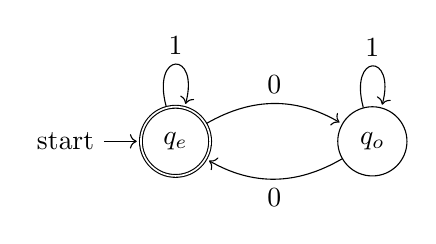
\begin{tikzpicture}[shorten >=1pt, node distance=2.5cm, on grid, auto]
  \node[state, initial, accepting] (qe) {$q_e$};
  \node[state] (qo) [right=of qe] {$q_o$};
  \path[->]
    (qe) edge[bend left] node {0} (qo)
    (qo) edge[bend left] node {0} (qe)
    (qe) edge[loop above] node {1} ()
    (qo) edge[loop above] node {1} ();
\end{tikzpicture}
\end{center}
\end{example}

\begin{example}
Write a regex for all binary strings that end with 01.

\emph{Solution.} $(0 \mid 1)^*01$

Any sequence of 0s and 1s, followed by 01.
\end{example}

\begin{example}
Construct a DFA for strings over $\{a, b\}$ containing no substring $bb$.

\emph{Solution.} Three states tracking what we've seen at the end:
\begin{itemize}
  \item $q_0$: Start, or last symbol was $a$ (no recent $b$)
  \item $q_1$: Last symbol was $b$
  \item $q_{\text{dead}}$: Saw $bb$, reject
\end{itemize}

\begin{itemize}
  \item From $q_0$: On $a$, stay in $q_0$. On $b$, go to $q_1$.
  \item From $q_1$: On $a$, go to $q_0$. On $b$, go to $q_{\text{dead}}$.
  \item From $q_{\text{dead}}$: Stay in $q_{\text{dead}}$ on any input.
  \item Accept states: $\{q_0, q_1\}$
\end{itemize}
\end{example}

\begin{example}
Prove that the intersection of two regular languages is regular.

\emph{Solution.} Let $L_1$ be recognized by DFA $M_1 = (Q_1, \Sigma, \delta_1, q_1, F_1)$ and let $L_2$ be recognized by $M_2 = (Q_2, \Sigma, \delta_2, q_2, F_2)$.

Construct the product DFA $M = (Q_1 \times Q_2, \Sigma, \delta, (q_1, q_2), F_1 \times F_2)$ where:
\[
\delta((p, q), a) = (\delta_1(p, a), \delta_2(q, a))
\]
This DFA accepts $w$ iff both $M_1$ and $M_2$ accept $w$, so $L(M) = L_1 \cap L_2$.
\end{example}

\begin{example}
Minimize the following DFA over $\{0, 1\}$.

States: $\{A, B, C, D\}$. Start: $A$. Accept: $\{C\}$.
Transitions: $\delta(A,0)=B$, $\delta(A,1)=C$, $\delta(B,0)=B$, $\delta(B,1)=C$, $\delta(C,0)=D$, $\delta(C,1)=C$, $\delta(D,0)=D$, $\delta(D,1)=C$.

\emph{Solution.} Using the table-filling algorithm:
\begin{enumerate}
  \item Mark $(A,C), (B,C), (D,C)$ (one accept, one non-accept).
  \item Check remaining pairs:
    \begin{itemize}
      \item $(A,B)$: $\delta(A,0)=B$, $\delta(B,0)=B$ --- same. $\delta(A,1)=C$, $\delta(B,1)=C$ --- same. Not distinguishable yet.
      \item $(A,D)$: $\delta(A,0)=B$, $\delta(D,0)=D$. Check $(B,D)$ first.
      \item $(B,D)$: $\delta(B,0)=B$, $\delta(D,0)=D$ --- need to check $(B,D)$. $\delta(B,1)=C$, $\delta(D,1)=C$ --- same. Not distinguishable.
    \end{itemize}
  \item States $A$, $B$, $D$ are equivalent. Merge them into one state.
\end{enumerate}
Minimal DFA has 2 states: $\{A,B,D\}$ and $\{C\}$.
\end{example}

\begin{example}
Prove that $L = \{0^n1^n : n \geq 0\}$ is not regular using the pumping lemma.

\emph{Proof.} Assume $L$ is regular. Let $p$ be the pumping length.

Choose $w = 0^p1^p \in L$. Then $|w| = 2p \geq p$.

By the pumping lemma, $w = xyz$ where $|y| > 0$, $|xy| \leq p$, and $xy^iz \in L$ for all $i$.

Since $|xy| \leq p$ and $w$ starts with $p$ zeros, $xy$ consists only of 0s. So $y = 0^k$ for some $k > 0$.

Consider $i = 2$: $xy^2z = 0^{p+k}1^p$. Since $k > 0$, this has more 0s than 1s, so $xy^2z \notin L$.

Contradiction. Therefore $L$ is not regular. \qed
\end{example}

\begin{example}
Write a regular expression for all binary strings with at least two 0s.

\emph{Solution.} We need at least two 0s, with any number of 0s and 1s before, between, and after them:
\[
(0 \mid 1)^* 0 (0 \mid 1)^* 0 (0 \mid 1)^*
\]
Equivalently, using $1^*$ instead of $(0 \mid 1)^*$ where appropriate: $1^* 0 1^* 0 (0 \mid 1)^*$ (but the first form is more symmetric).
\end{example}

\begin{example}
Design a DFA over $\{a, b\}$ that accepts strings where the number of $a$s is divisible by 3.

\emph{Solution.} Track $(\text{number of } a\text{s}) \mod 3$. Three states: $q_0$ (seen $0 \mod 3$), $q_1$ (seen $1 \mod 3$), $q_2$ (seen $2 \mod 3$).
\begin{itemize}
  \item Start state: $q_0$ (zero $a$s)
  \item Accept state: $\{q_0\}$ (divisible by 3)
  \item Transitions on $a$: $q_0 \to q_1 \to q_2 \to q_0$ (cycle)
  \item Transitions on $b$: self-loops (don't change count)
\end{itemize}

Formally: $\delta(q_i, a) = q_{(i+1) \mod 3}$ and $\delta(q_i, b) = q_i$.
\end{example}

\begin{example}
Prove that $L = \{ww : w \in \{0,1\}^*\}$ is not regular.

\emph{Proof.} Assume $L$ is regular with pumping length $p$.

Choose $s = 0^p 1 0^p 1 \in L$ (where $w = 0^p 1$). We have $|s| = 2p + 2 \geq p$.

By the pumping lemma, $s = xyz$ with $|y| > 0$, $|xy| \leq p$.

Since $|xy| \leq p$ and $s$ starts with $p$ zeros, we have $y = 0^k$ for some $k \geq 1$.

Consider $xy^0z = 0^{p-k} 1 0^p 1$. The first half has $p - k$ zeros before its first 1, while the second half has $p$ zeros before its first 1. Since $k \geq 1$, these halves are different, so $xy^0z \notin L$.

Contradiction. Therefore $L$ is not regular. \qed
\end{example}

\begin{example}
Design a DFA for binary strings representing numbers divisible by 3 (reading left to right, most significant bit first).

\emph{Solution.} Track the value $\mod 3$ as we read. If current value is $v$ and we read bit $b$, new value is $2v + b \pmod 3$.

States: $q_0, q_1, q_2$ representing value $\mod 3$.
\begin{itemize}
  \item Start: $q_0$ (value 0)
  \item Accept: $\{q_0\}$
  \item From $q_0$: on 0, $2 \cdot 0 + 0 = 0 \to q_0$; on 1, $2 \cdot 0 + 1 = 1 \to q_1$
  \item From $q_1$: on 0, $2 \cdot 1 + 0 = 2 \to q_2$; on 1, $2 \cdot 1 + 1 = 3 \equiv 0 \to q_0$
  \item From $q_2$: on 0, $2 \cdot 2 + 0 = 4 \equiv 1 \to q_1$; on 1, $2 \cdot 2 + 1 = 5 \equiv 2 \to q_2$
\end{itemize}

Test: $110_2 = 6$. Path: $q_0 \xrightarrow{1} q_1 \xrightarrow{1} q_0 \xrightarrow{0} q_0$. Accept. \checkmark
\end{example}

\begin{commonmistake}
\textbf{Confusing $\emptyset$ and $\varepsilon$.} $\emptyset$ is the regex for the empty language (no strings). $\varepsilon$ is the regex for the language containing only the empty string $\{\varepsilon\}$.
\end{commonmistake}

\begin{commonmistake}
\textbf{Forgetting that the pumping lemma is only for proving non-regularity.} You cannot use it to prove a language IS regular. Satisfying the pumping lemma is necessary but not sufficient for regularity.
\end{commonmistake}

\begin{goingdeeper}[Going Deeper: Duality and Observation]
Week 8 introduced \emph{initial algebras} for understanding recursive data structures like trees. This week, we glimpse the dual concept: \emph{coalgebras} for understanding systems with observable behavior, like automata.

\subsubsection*{Algebras vs Coalgebras}

Recall from Week 8: an algebra takes us \emph{from} structure \emph{to} a set:
\begin{itemize}
  \item List algebra: $([], \text{cons})$ tells how to \emph{build} lists
  \item Tree algebra: $(\text{leaf}, \text{node})$ tells how to \emph{build} trees
  \item The arrow points ``inward'': $F(A) \to A$
\end{itemize}

A \emph{coalgebra} reverses the direction---it tells us how to \emph{observe} or \emph{decompose}:
\begin{itemize}
  \item The arrow points ``outward'': $A \to F(A)$
  \item Given a state, we observe something about it
\end{itemize}

\subsubsection*{DFAs as Coalgebras}

A DFA has a transition function and acceptance condition. For each state $q$, we can observe:
\begin{enumerate}
  \item Is $q$ accepting? (Output: yes/no)
  \item Where do we go on each input symbol? (Transitions)
\end{enumerate}

This gives a function: $\text{state} \to (\text{output} \times \text{next-states})$.

Formally, a DFA over alphabet $\Sigma$ is a coalgebra for the pattern:
\[
Q \to \{0, 1\} \times Q^\Sigma
\]
where $Q^\Sigma$ means ``a function from $\Sigma$ to $Q$.''

\subsubsection*{Streams: Another Coalgebra}

An infinite stream of values from $A$ can be observed:
\begin{enumerate}
  \item What's the first element? (The head)
  \item What's the rest of the stream? (The tail)
\end{enumerate}

This gives: $\text{Stream}(A) \to A \times \text{Stream}(A)$.

Contrast with lists: for lists, we have $1 + A \times \text{List}(A) \to \text{List}(A)$ (building up from $[]$ and $\text{cons}$).

For streams, we have $\text{Stream}(A) \to A \times \text{Stream}(A)$ (tearing down into head and tail).

\subsubsection*{The Duality Pattern}

\begin{center}
\begin{tabular}{lcc}
& \textbf{Algebra} & \textbf{Coalgebra} \\
\hline
Structure map & $F(A) \to A$ & $A \to F(A)$ \\
Intuition & Constructors & Observers \\
Universal object & Initial (smallest) & Final (largest) \\
Universal map & Fold (catamorphism) & Unfold (anamorphism) \\
Data & Finite & Potentially infinite \\
Example & Lists, trees & Streams, automata \\
\end{tabular}
\end{center}

\subsubsection*{Bisimulation: When Are Two States ``The Same''?}

Two DFA states are \emph{bisimilar} if no sequence of observations can distinguish them. This means:
\begin{itemize}
  \item They give the same accept/reject output
  \item For each input symbol, they transition to bisimilar states
\end{itemize}

This is exactly what DFA minimization does: merge bisimilar states!

\subsubsection*{Exercises: Duality and Observation}

\begin{enumerate}
  \item For an infinite stream, what is $\text{head}(\text{tail}(\text{tail}([0, 1, 2, 3, \ldots])))$?

  \item The Fibonacci stream is $[0, 1, 1, 2, 3, 5, 8, \ldots]$. If we define it by $\text{fib} = [0, 1] \mathbin{+\!\!+} \text{zipWith}(+, \text{fib}, \text{tail}(\text{fib}))$, what are the first 5 elements? (Trace through.)

  \item For the DFA from the ``even number of 0s'' example, write out the coalgebra structure: for each state, give the pair $(\text{accept?}, \text{transitions})$.

  \item Fill in this duality table:
  \begin{center}
  \begin{tabular}{lcc}
  \textbf{Concept} & \textbf{Algebra} & \textbf{Coalgebra} \\
  \hline
  Structure map & $F(A) \to A$ & ? \\
  Constructors & Build up & ? \\
  Universal object & Initial & ? \\
  Universal map & Fold & ? \\
  Data type & Finite & ?
  \end{tabular}
  \end{center}

  \item Why can we have infinite streams but (in a total language) not ``infinite lists''? (Hint: What goes wrong if we try to fold over an infinite structure?)

  \item In the DFA minimization example, states $A$, $B$, $D$ were merged because they were bisimilar. Verify that $A$ and $B$ are bisimilar by checking: (a) same accept status, (b) transitions lead to bisimilar states.

  \item \textbf{Challenge:} The ``Brzozowski derivative'' of a language $L$ with respect to symbol $a$ is $\partial_a(L) = \{w : aw \in L\}$. Show that this is exactly the ``observe a transition'' operation in the coalgebra view of languages.
\end{enumerate}
\end{goingdeeper}

\subsection*{Practice}
\begin{enumerate}
  \item Write a regex for all binary strings that end with 01.

  \item Construct a DFA for strings over $\{a, b\}$ that contain no substring $bb$.

  \item Minimize a DFA with 4 states of your choosing.

  \item Prove that the intersection of two regular languages is regular.

  \item Write a regex for binary strings with at least two 0s.

  \item Design a DFA that accepts strings over $\{a,b\}$ where the number of $a$s is divisible by 3.

  \item Prove that $L = \{w \in \{0,1\}^* : w = w^R\}$ (palindromes) is not regular.

  \item Convert the regex $(a \mid b)^*aba$ to an NFA.

  \item Show that if $L$ is regular, then $L^R = \{w^R : w \in L\}$ is regular.

  \item Design a DFA for binary strings representing numbers divisible by 3.

  \item Prove that $L = \{a^{n^2} : n \geq 0\}$ is not regular.

  \item Given DFAs for $L_1$ and $L_2$, construct a DFA for $L_1 \setminus L_2$.
\end{enumerate}

\newpage
\section{Week 10: Analysis of Algorithm Efficiency}
\subsection*{Reading}
Epp \S 11.1--11.5.\\
\textbf{Category theory companion:} Week 10 (\texttt{category\_theory\_companion.pdf}).

\subsection*{Learning objectives}
\begin{itemize}
  \item Compare growth rates of functions using limits and dominance.
  \item Apply big-$O$, big-$\Omega$, and big-$\Theta$ notation correctly.
  \item Analyze the time complexity of loops and nested loops.
  \item Solve recurrences using expansion, substitution, and the master theorem.
  \item Classify algorithms by their complexity class.
\end{itemize}

\subsection*{Key definitions and facts}

\begin{definition}[Asymptotic notation]
Let $f, g: \N \to \R^+$ be functions.

\textbf{Big-O (upper bound):} $f(n) = O(g(n))$ if there exist constants $c > 0$ and $n_0$ such that:
\[
f(n) \leq c \cdot g(n) \quad \text{for all } n \geq n_0
\]

\textbf{Big-Omega (lower bound):} $f(n) = \Omega(g(n))$ if there exist constants $c > 0$ and $n_0$ such that:
\[
f(n) \geq c \cdot g(n) \quad \text{for all } n \geq n_0
\]

\textbf{Big-Theta (tight bound):} $f(n) = \Theta(g(n))$ if $f(n) = O(g(n))$ and $f(n) = \Omega(g(n))$.
\end{definition}

\begin{theorem}[Limit test for asymptotic notation]
If $\lim_{n \to \infty} \frac{f(n)}{g(n)} = L$, then:
\begin{itemize}
  \item $L = 0 \Rightarrow f(n) = O(g(n))$ but $f(n) \neq \Theta(g(n))$
  \item $0 < L < \infty \Rightarrow f(n) = \Theta(g(n))$
  \item $L = \infty \Rightarrow f(n) = \Omega(g(n))$ but $f(n) \neq O(g(n))$
\end{itemize}
\end{theorem}

\begin{definition}[Little-o and little-omega]
\textbf{Little-o:} $f(n) = o(g(n))$ if $\lim_{n \to \infty} \frac{f(n)}{g(n)} = 0$. This means $f$ grows strictly slower than $g$.

\textbf{Little-omega:} $f(n) = \omega(g(n))$ if $\lim_{n \to \infty} \frac{f(n)}{g(n)} = \infty$. This means $f$ grows strictly faster than $g$.
\end{definition}

\begin{theorem}[Properties of asymptotic notation]
\begin{enumerate}
  \item \textbf{Transitivity:} If $f = O(g)$ and $g = O(h)$, then $f = O(h)$.
  \item \textbf{Reflexivity:} $f = O(f)$, $f = \Omega(f)$, $f = \Theta(f)$.
  \item \textbf{Symmetry:} $f = \Theta(g)$ iff $g = \Theta(f)$.
  \item \textbf{Transpose symmetry:} $f = O(g)$ iff $g = \Omega(f)$.
  \item \textbf{Sum rule:} $O(f) + O(g) = O(\max(f, g))$.
  \item \textbf{Product rule:} $O(f) \cdot O(g) = O(f \cdot g)$.
  \item \textbf{Constant factors:} $O(cf) = O(f)$ for any constant $c > 0$.
\end{enumerate}
\end{theorem}

\subsection*{Common complexity classes}

\begin{definition}[Growth rate hierarchy]
Listed from slowest to fastest growth:
\[
O(1) \subset O(\log n) \subset O(\sqrt{n}) \subset O(n) \subset O(n \log n) \subset O(n^2) \subset O(n^3) \subset O(2^n) \subset O(n!)
\]
\end{definition}

\begin{center}
\begin{tabular}{lll}
\textbf{Notation} & \textbf{Name} & \textbf{Example} \\
\hline
$O(1)$ & Constant & Array access \\
$O(\log n)$ & Logarithmic & Binary search \\
$O(n)$ & Linear & Linear search \\
$O(n \log n)$ & Linearithmic & Merge sort \\
$O(n^2)$ & Quadratic & Bubble sort \\
$O(n^3)$ & Cubic & Matrix multiplication (naive) \\
$O(2^n)$ & Exponential & Subset enumeration \\
$O(n!)$ & Factorial & Permutation enumeration \\
\end{tabular}
\end{center}

\subsection*{Analyzing code}

\begin{theorem}[Loop analysis]
\begin{itemize}
  \item A loop that runs $n$ times with $O(1)$ body: $O(n)$
  \item Two nested loops, each running $n$ times: $O(n^2)$
  \item Three nested loops, each running $n$ times: $O(n^3)$
  \item A loop that halves the problem size each iteration: $O(\log n)$
\end{itemize}
\end{theorem}

\begin{strategy}
To analyze a loop:
\begin{enumerate}
  \item Count how many times the loop body executes.
  \item Multiply by the cost of one iteration.
  \item For nested loops, multiply the counts of each level.
\end{enumerate}
\end{strategy}

\begin{theorem}[Summation formulas]
\begin{align*}
\sum_{i=1}^n 1 &= n \\
\sum_{i=1}^n i &= \frac{n(n+1)}{2} = \Theta(n^2) \\
\sum_{i=1}^n i^2 &= \frac{n(n+1)(2n+1)}{6} = \Theta(n^3) \\
\sum_{i=0}^n r^i &= \frac{r^{n+1} - 1}{r - 1} = \Theta(r^n) \text{ for } r > 1 \\
\sum_{i=1}^n \frac{1}{i} &= \Theta(\log n) \text{ (harmonic series)}
\end{align*}
\end{theorem}

\subsection*{Recurrence relations}

\begin{definition}[Recurrence relation]
A \textbf{recurrence relation} expresses $T(n)$ in terms of $T$ applied to smaller inputs. Common form for divide-and-conquer:
\[
T(n) = aT(n/b) + f(n)
\]
where $a \geq 1$ is the number of subproblems, $n/b$ is the subproblem size, and $f(n)$ is the work outside the recursive calls.
\end{definition}

\begin{theorem}[Master theorem]
For recurrence $T(n) = aT(n/b) + f(n)$ where $a \geq 1$, $b > 1$:

Let $c = \log_b a$. Compare $f(n)$ with $n^c$:

\textbf{Case 1:} If $f(n) = O(n^{c - \epsilon})$ for some $\epsilon > 0$, then $T(n) = \Theta(n^c)$.

\textbf{Case 2:} If $f(n) = \Theta(n^c \log^k n)$ for some $k \geq 0$, then $T(n) = \Theta(n^c \log^{k+1} n)$.

\textbf{Case 3:} If $f(n) = \Omega(n^{c + \epsilon})$ for some $\epsilon > 0$ and $af(n/b) \leq kf(n)$ for some $k < 1$, then $T(n) = \Theta(f(n))$.
\end{theorem}

\begin{theorem}[Common recurrences]
\begin{center}
\begin{tabular}{lll}
\textbf{Recurrence} & \textbf{Solution} & \textbf{Example} \\
\hline
$T(n) = T(n/2) + O(1)$ & $O(\log n)$ & Binary search \\
$T(n) = T(n-1) + O(1)$ & $O(n)$ & Linear recursion \\
$T(n) = T(n-1) + O(n)$ & $O(n^2)$ & Selection sort \\
$T(n) = 2T(n/2) + O(1)$ & $O(n)$ & Tree traversal \\
$T(n) = 2T(n/2) + O(n)$ & $O(n \log n)$ & Merge sort \\
$T(n) = 2T(n-1) + O(1)$ & $O(2^n)$ & Fibonacci (naive) \\
\end{tabular}
\end{center}
\end{theorem}

\subsection*{Solving recurrences}

\begin{strategy}
\textbf{Method 1: Expansion (iteration)}
\begin{enumerate}
  \item Expand the recurrence several times.
  \item Identify the pattern.
  \item Sum the terms.
\end{enumerate}

\textbf{Method 2: Substitution (guess and verify)}
\begin{enumerate}
  \item Guess the form of the solution.
  \item Use induction to verify.
  \item Adjust constants as needed.
\end{enumerate}

\textbf{Method 3: Master theorem}
\begin{enumerate}
  \item Identify $a$, $b$, and $f(n)$.
  \item Compute $c = \log_b a$.
  \item Determine which case applies.
\end{enumerate}
\end{strategy}

\subsection*{Best, worst, and average case}

\begin{definition}[Case analysis]
\begin{itemize}
  \item \textbf{Worst case:} Maximum time over all inputs of size $n$.
  \item \textbf{Best case:} Minimum time over all inputs of size $n$.
  \item \textbf{Average case:} Expected time over a probability distribution on inputs.
\end{itemize}
Usually, we report worst-case complexity.
\end{definition}

\subsection*{Complexity classes and reductions}

\begin{definition}[Decision problem]
A \textbf{decision problem} has a yes/no answer for each input. Complexity classes are typically defined for decision problems.
\end{definition}

\begin{definition}[Classes P and NP]
\begin{itemize}
  \item $\mathbf{P}$: problems solvable in polynomial time by a deterministic algorithm.
  \item $\mathbf{NP}$: problems whose solutions can be \emph{verified} in polynomial time (equivalently, solvable by a nondeterministic polynomial-time algorithm).
\end{itemize}
\end{definition}

\begin{definition}[Reductions, NP-hard, NP-complete]
A polynomial-time reduction from $A$ to $B$ (written $A \leq_p B$) transforms instances of $A$ into instances of $B$ preserving yes/no answers.
\begin{itemize}
  \item $B$ is \textbf{NP-hard} if every problem in NP reduces to $B$.
  \item $B$ is \textbf{NP-complete} if $B \in \textbf{NP}$ and $B$ is NP-hard.
\end{itemize}
\end{definition}

\begin{strategy}
To prove a problem $B$ is NP-complete:
\begin{enumerate}
  \item Show $B \in \mathbf{NP}$ (solutions are verifiable in poly time).
  \item Reduce a known NP-complete problem $A$ to $B$ in polynomial time.
\end{enumerate}
\end{strategy}

\begin{example}[Common NP-complete problems]
SAT, 3-SAT, CLIQUE, VERTEX COVER, HAMILTONIAN CYCLE, and SUBSET SUM are all NP-complete.
\end{example}

\subsection*{Worked examples}

\begin{example}
Show that $3n^2 + 5n + 7 = \Theta(n^2)$.

\emph{Solution.}

\textbf{Upper bound:} For $n \geq 1$: $3n^2 + 5n + 7 \leq 3n^2 + 5n^2 + 7n^2 = 15n^2$. So $3n^2 + 5n + 7 = O(n^2)$ with $c = 15$, $n_0 = 1$.

\textbf{Lower bound:} For $n \geq 1$: $3n^2 + 5n + 7 \geq 3n^2$. So $3n^2 + 5n + 7 = \Omega(n^2)$ with $c = 3$, $n_0 = 1$.

Therefore $3n^2 + 5n + 7 = \Theta(n^2)$.
\end{example}

\begin{example}
Order the functions $n \log n$, $n^{1.5}$, $2^n$, $n^3$ by growth rate.

\emph{Solution.} Compare using limits:
\begin{itemize}
  \item $\lim_{n \to \infty} \frac{n \log n}{n^{1.5}} = \lim_{n \to \infty} \frac{\log n}{\sqrt{n}} = 0$ (L'Hôpital's). So $n \log n = o(n^{1.5})$.
  \item $\lim_{n \to \infty} \frac{n^{1.5}}{n^3} = \lim_{n \to \infty} \frac{1}{n^{1.5}} = 0$. So $n^{1.5} = o(n^3)$.
  \item $\lim_{n \to \infty} \frac{n^3}{2^n} = 0$ (exponential dominates polynomial). So $n^3 = o(2^n)$.
\end{itemize}

Order (slowest to fastest): $n \log n \prec n^{1.5} \prec n^3 \prec 2^n$.
\end{example}

\begin{example}
Analyze the runtime of nested loops:
\begin{verbatim}
for i = 1 to n:
    for j = 1 to n:
        // O(1) operation
\end{verbatim}

\emph{Solution.} The inner loop runs $n$ times for each of $n$ iterations of the outer loop. Total iterations: $n \times n = n^2$. Each iteration is $O(1)$. Total: $O(n^2)$.
\end{example}

\begin{example}
Analyze the runtime:
\begin{verbatim}
for i = 1 to n:
    for j = 1 to i:
        // O(1) operation
\end{verbatim}

\emph{Solution.} The inner loop runs $i$ times. Total iterations:
\[
\sum_{i=1}^n i = \frac{n(n+1)}{2} = \Theta(n^2)
\]
\end{example}

\begin{example}
Solve the recurrence $T(n) = 2T(n/2) + n$ with $T(1) = 1$.

\emph{Solution (Master theorem).} Here $a = 2$, $b = 2$, $f(n) = n$.

$c = \log_b a = \log_2 2 = 1$, so $n^c = n$.

Compare: $f(n) = n = \Theta(n^1) = \Theta(n^c \log^0 n)$.

This is Case 2 with $k = 0$: $T(n) = \Theta(n^c \log^{k+1} n) = \Theta(n \log n)$.
\end{example}

\begin{example}
Solve $T(n) = 2T(n/2) + n$ by expansion.

\emph{Solution.}
\begin{align*}
T(n) &= 2T(n/2) + n \\
     &= 2[2T(n/4) + n/2] + n = 4T(n/4) + 2n \\
     &= 4[2T(n/8) + n/4] + 2n = 8T(n/8) + 3n \\
     &\vdots \\
     &= 2^k T(n/2^k) + kn
\end{align*}

When $n/2^k = 1$, we have $k = \log_2 n$ and $T(1) = 1$:
\[
T(n) = 2^{\log n} \cdot 1 + n \log n = n + n \log n = \Theta(n \log n)
\]
\end{example}

\begin{example}
Analyze the runtime of binary search.

\emph{Solution.} At each step, the search space is halved. If $T(n)$ is the time for a search in an array of size $n$:
\[
T(n) = T(n/2) + O(1), \quad T(1) = O(1)
\]
By Master theorem: $a = 1$, $b = 2$, $f(n) = O(1)$.
$c = \log_2 1 = 0$, so $n^c = 1$.
$f(n) = O(1) = \Theta(n^0)$. Case 2 with $k = 0$: $T(n) = \Theta(\log n)$.
\end{example}

\begin{example}
Show that $\log(n!) = \Theta(n \log n)$.

\emph{Solution.}

\textbf{Upper bound:} $n! = 1 \cdot 2 \cdots n \leq n^n$, so $\log(n!) \leq n \log n$.

\textbf{Lower bound:} $n! = 1 \cdot 2 \cdots n \geq (n/2)^{n/2}$ (considering only the largest $n/2$ terms), so:
\[
\log(n!) \geq \frac{n}{2} \log \frac{n}{2} = \frac{n}{2} (\log n - 1) = \Omega(n \log n)
\]

Therefore $\log(n!) = \Theta(n \log n)$.
\end{example}

\begin{example}
Prove that $\log n = O(n^\epsilon)$ for any $\epsilon > 0$.

\emph{Proof.} Use the limit test:
\[
\lim_{n \to \infty} \frac{\log n}{n^\epsilon}
\]
This is an $\infty/\infty$ form, so apply L'Hôpital's rule:
\[
\lim_{n \to \infty} \frac{1/n}{\epsilon n^{\epsilon - 1}} = \lim_{n \to \infty} \frac{1}{\epsilon n^\epsilon} = 0
\]
Since the limit is 0, we have $\log n = O(n^\epsilon)$. In fact, $\log n = o(n^\epsilon)$, meaning log grows strictly slower than any positive power of $n$.
\end{example}

\begin{example}
Show that $2^{n+1} = \Theta(2^n)$ but $2^{2n} \neq O(2^n)$.

\emph{Solution.}

\textbf{Part 1:} $2^{n+1} = 2 \cdot 2^n$. So $2^{n+1} \leq 2 \cdot 2^n$ (with $c = 2$) and $2^{n+1} \geq 2 \cdot 2^n$ (with $c = 2$). Thus $2^{n+1} = \Theta(2^n)$.

\textbf{Part 2:} $2^{2n} = (2^2)^n = 4^n$. Check if $4^n = O(2^n)$:
\[
\lim_{n \to \infty} \frac{4^n}{2^n} = \lim_{n \to \infty} 2^n = \infty
\]
Since the limit is $\infty$, $4^n$ grows faster than $2^n$, so $2^{2n} \neq O(2^n)$.

\textbf{Intuition:} Constant factors in the exponent matter! $2^{cn}$ for $c > 1$ is exponentially larger than $2^n$.
\end{example}

\begin{example}
Solve $T(n) = 3T(n/2) + n$ using the Master theorem.

\emph{Solution.} Identify: $a = 3$, $b = 2$, $f(n) = n$.

Compute $c = \log_b a = \log_2 3 \approx 1.585$.

Compare $f(n) = n = n^1$ with $n^c = n^{1.585}$.

Since $1 < 1.585$, we have $f(n) = O(n^{c - \epsilon})$ for $\epsilon = 0.585$.

This is \textbf{Case 1}: $T(n) = \Theta(n^c) = \Theta(n^{\log_2 3})$.
\end{example}

\begin{example}
Analyze the time complexity of this code:
\begin{verbatim}
for i = 1 to n:
    for j = i to n:
        // O(1) work
\end{verbatim}

\emph{Solution.} The inner loop runs $n - i + 1$ times for each $i$. Total iterations:
\[
\sum_{i=1}^{n} (n - i + 1) = \sum_{k=1}^{n} k = \frac{n(n+1)}{2} = \Theta(n^2)
\]
(Substituted $k = n - i + 1$.)
\end{example}

\begin{example}
Solve the recurrence $T(n) = T(n-1) + n$ by expansion.

\emph{Solution.} Expand:
\begin{align*}
T(n) &= T(n-1) + n \\
     &= T(n-2) + (n-1) + n \\
     &= T(n-3) + (n-2) + (n-1) + n \\
     &\vdots \\
     &= T(1) + 2 + 3 + \cdots + n \\
     &= T(1) + \sum_{k=2}^{n} k = T(1) + \frac{n(n+1)}{2} - 1
\end{align*}
If $T(1) = 1$: $T(n) = \frac{n(n+1)}{2} = \Theta(n^2)$.
\end{example}

\begin{commonmistake}
\textbf{Treating big-O as equality.} $f = O(g)$ means $f$ is bounded above by $g$, not equal to it. Better to read as ``$f$ is $O(g)$'' rather than ``$f$ equals $O(g)$.''
\end{commonmistake}

\begin{commonmistake}
\textbf{Confusing worst-case and big-O.} Big-O describes an upper bound on a function. Worst-case describes the maximum over inputs. They're related but distinct concepts.
\end{commonmistake}

\begin{commonmistake}
\textbf{Ignoring the regularity condition in Master theorem Case 3.} Case 3 requires $af(n/b) \leq kf(n)$ for some $k < 1$. This is usually satisfied but should be checked.
\end{commonmistake}

%% ================================================================
%% GOING DEEPER: Monoids—Categories with One Object
%% ================================================================
\begin{goingdeeper}[Going Deeper: Monoids—Categories with One Object]

Throughout this course, we've seen how categories unify different areas of mathematics. We end with a beautiful observation: \emph{monoids are categories with exactly one object}.
For more detail, see the Category Theory Companion, Week 10.

\subsubsection*{Monoids: The Definition}

A \textbf{monoid} $(M, \cdot, e)$ is a set $M$ equipped with:
\begin{itemize}
  \item A binary operation $\cdot : M \times M \to M$
  \item An identity element $e \in M$
\end{itemize}
satisfying:
\begin{itemize}
  \item \textbf{Associativity:} $(a \cdot b) \cdot c = a \cdot (b \cdot c)$ for all $a, b, c \in M$
  \item \textbf{Identity:} $e \cdot a = a = a \cdot e$ for all $a \in M$
\end{itemize}

Compare this to the axioms for a category:
\[
\begin{array}{c|c}
\textbf{Monoid} & \textbf{Category} \\
\hline
\text{Elements of } M & \text{Morphisms} \\
\text{Multiplication } \cdot & \text{Composition } \circ \\
\text{Identity } e & \text{Identity morphism } \id \\
\text{Associativity of } \cdot & \text{Associativity of } \circ \\
\end{array}
\]

If a category has only one object $\star$, then \emph{all} morphisms go from $\star$ to $\star$—they can always be composed! The morphisms form a monoid under composition.

\begin{center}
\begin{tikzcd}[row sep=small, column sep=small]
& \star \arrow[loop above, "e", distance=2em]
       \arrow[loop left, "a"', distance=2em]
       \arrow[loop right, "b", distance=2em]
       \arrow[loop below, "ab"', distance=2em]
\end{tikzcd}
\end{center}

\subsubsection*{Examples of Monoids}

\textbf{1. Natural numbers under addition:} $(\N, +, 0)$
\begin{itemize}
  \item Elements: $0, 1, 2, 3, \ldots$
  \item Operation: addition
  \item Identity: 0 (since $0 + n = n = n + 0$)
\end{itemize}

\textbf{2. Natural numbers under multiplication:} $(\N, \times, 1)$
\begin{itemize}
  \item Same set, different monoid structure!
  \item Identity: 1 (since $1 \times n = n = n \times 1$)
\end{itemize}

\textbf{3. Strings under concatenation:} $(\Sigma^*, \cdot, \varepsilon)$
\begin{itemize}
  \item Elements: all strings over alphabet $\Sigma$
  \item Operation: concatenation (e.g., ``$ab$'' $\cdot$ ``$cd$'' $=$ ``$abcd$'')
  \item Identity: empty string $\varepsilon$
\end{itemize}

\textbf{4. Functions under composition:} $(A \to A, \circ, \id_A)$
\begin{itemize}
  \item Elements: functions from $A$ to itself
  \item Operation: function composition
  \item Identity: the identity function
\end{itemize}

\textbf{5. Complexity classes:} The big-$O$ notation satisfies monoid-like properties:
\begin{itemize}
  \item $O(f) \cdot O(g) = O(f \cdot g)$ (product rule)
  \item $O(1)$ acts as a multiplicative identity
\end{itemize}

\subsubsection*{The Free Monoid}

Given any set $\Sigma$ (an ``alphabet''), we can form the \textbf{free monoid} $\Sigma^*$: the set of all finite strings over $\Sigma$, with concatenation as the operation.

Why ``free''? Because $\Sigma^*$ is the \emph{most general} monoid generated by $\Sigma$—it satisfies no equations other than the monoid axioms. This is a \textbf{universal property}:

\begin{quote}
For any monoid $M$ and any function $f: \Sigma \to M$, there is a \emph{unique} monoid homomorphism $\bar{f}: \Sigma^* \to M$ extending $f$.
\end{quote}

\[
\begin{tikzcd}
\Sigma \arrow[r, "f"] \arrow[d, hook, "\eta"'] & M \\
\Sigma^* \arrow[ur, dashed, "\exists! \bar{f}"']
\end{tikzcd}
\]

The map $\eta: \Sigma \to \Sigma^*$ sends each letter to the one-letter string.

\textbf{Example.} Let $\Sigma = \{a, b\}$ and let $M = (\N, +, 0)$. Define $f(a) = 3$, $f(b) = 5$. The unique extension $\bar{f}: \Sigma^* \to \N$ maps each string to the sum of its letter values:
\[
\bar{f}(aabba) = f(a) + f(a) + f(b) + f(b) + f(a) = 3 + 3 + 5 + 5 + 3 = 19
\]

This is why $\Sigma^*$ appears in automata theory: a DFA computes exactly a monoid homomorphism from the free monoid to a finite monoid!

\subsubsection*{Monoid Homomorphisms}

A \textbf{monoid homomorphism} $\phi: (M, \cdot_M, e_M) \to (N, \cdot_N, e_N)$ is a function $\phi: M \to N$ satisfying:
\begin{itemize}
  \item $\phi(a \cdot_M b) = \phi(a) \cdot_N \phi(b)$ \quad (preserves multiplication)
  \item $\phi(e_M) = e_N$ \quad (preserves identity)
\end{itemize}

In categorical terms: a homomorphism between one-object categories is exactly a \textbf{functor}!

\textbf{Example.} The length function $\text{len}: \Sigma^* \to \N$ is a monoid homomorphism from $(\Sigma^*, \cdot, \varepsilon)$ to $(\N, +, 0)$:
\begin{itemize}
  \item $\text{len}(s \cdot t) = \text{len}(s) + \text{len}(t)$
  \item $\text{len}(\varepsilon) = 0$
\end{itemize}

\textbf{Example.} The determinant function $\det: \text{GL}_n(\R) \to \R^*$ is a monoid homomorphism:
\begin{itemize}
  \item $\det(AB) = \det(A) \cdot \det(B)$
  \item $\det(I) = 1$
\end{itemize}

\subsubsection*{Connection to Complexity Analysis}

Consider the monoid $(\N, +, 0)$ of running times. When we analyze:
\[
T(n) = T(n/2) + O(1)
\]
we're saying: the total time is the \emph{sum} (monoid operation) of the recursive time plus the local work. The structure of recurrence relations reflects monoid structure!

For divide-and-conquer with $a$ subproblems:
\[
T(n) = \underbrace{T(n/b) + T(n/b) + \cdots + T(n/b)}_{a \text{ terms}} + f(n)
\]
The $a$-fold sum uses the monoid structure repeatedly.

\subsubsection*{Exercises: Monoids and Structure}

\begin{enumerate}
\item Verify that $(\Z, +, 0)$ is a monoid. Is $(\Z, -, 0)$ a monoid? Why or why not?

\item The set $\{0, 1\}$ with operation ``OR'' ($\lor$) and identity 0 forms a monoid. Write out its multiplication table.

\item Show that the set of $n \times n$ matrices over $\R$ with matrix multiplication and the identity matrix $I$ forms a monoid. (Note: this is \emph{not} a group—why?)

\item Let $\Sigma = \{0, 1\}$. The \emph{run-length encoding} maps a string to the sequence of run lengths. For example: $00111001 \mapsto [2, 3, 2, 1]$. Is run-length encoding a monoid homomorphism? Prove or give a counterexample.

\item \textbf{(Important)} Prove that if $\phi: M \to N$ is a monoid homomorphism, then the image $\phi(M) = \{\phi(m) : m \in M\}$ is a submonoid of $N$.

\item Let $\text{End}(A)$ be the monoid of functions $A \to A$ under composition. If $|A| = n$, what is $|\text{End}(A)|$? What is the identity element?

\item Consider the monoid $(\{0, 1, 2, \ldots, n-1\}, +_n, 0)$ where $+_n$ is addition mod $n$. Define a map $\phi: \Z \to \Z_n$ by $\phi(k) = k \mod n$. Prove this is a monoid homomorphism.

\item \textbf{(Challenge)} The powerset $\mathcal{P}(A)$ forms a monoid under union with $\emptyset$ as identity. It also forms a monoid under intersection with $A$ as identity. Are these monoids isomorphic? (Two monoids are isomorphic if there's a bijective homomorphism between them.)

\item \textbf{(Big-$O$ as Monoid)} Define a relation on functions where $f \sim g$ iff $f = \Theta(g)$. Show that the equivalence classes under $\sim$ form a monoid with multiplication $[f] \cdot [g] = [f \cdot g]$. What is the identity?

\item \textbf{(Connection to Automata)} Recall from Week 9 that a DFA defines a transition function $\delta: Q \times \Sigma \to Q$. Extend this to $\hat{\delta}: Q \times \Sigma^* \to Q$ by:
\begin{itemize}
  \item $\hat{\delta}(q, \varepsilon) = q$
  \item $\hat{\delta}(q, wa) = \delta(\hat{\delta}(q, w), a)$
\end{itemize}
Fix a state $q_0$. Show that the map $w \mapsto \hat{\delta}(q_0, -)$ gives a monoid homomorphism from $\Sigma^*$ to the monoid of functions $Q \to Q$.
\end{enumerate}

\subsubsection*{The Categorical Perspective: Full Circle}

We began this course with sets and functions, introduced diagrams to visualize composition, and discovered that many structures (preorders, graphs, automata) can be viewed categorically. Now we see that even the simplest algebraic structure—a monoid—is secretly a category.

This suggests a powerful principle: \emph{category theory doesn't replace other mathematics; it reveals the common structure underlying diverse areas}. The monoid of complexity classes, the monoid of string concatenation in automata theory, and the monoid of functions under composition are all instances of the same abstract pattern.

As you continue in computer science and mathematics, you'll encounter this pattern repeatedly:
\begin{itemize}
  \item Types form categories (where morphisms are functions)
  \item Proofs form categories (where morphisms witness logical entailment)
  \item Programs form categories (where morphisms are computations)
\end{itemize}

The tools you've developed—diagrams, universal properties, functors—are the beginning of a rich vocabulary for understanding computation, logic, and mathematics as aspects of a unified whole.

\end{goingdeeper}

\subsection*{Practice}
\begin{enumerate}
  \item Order the functions $n \log n$, $n^{1.5}$, $2^n$, $n^3$ by growth rate.

  \item Show that $3n^2 + 5n + 7$ is $\Theta(n^2)$.

  \item Solve the recurrence $T(n) = 2T(n/2) + n$ with $T(1) = 1$.

  \item Analyze the runtime of binary search.

  \item Prove: $\log n = O(n^\epsilon)$ for any $\epsilon > 0$.

  \item Analyze the complexity of:
\begin{verbatim}
for i = 1 to n:
    for j = i to n:
        for k = 1 to j:
            // O(1)
\end{verbatim}

  \item Solve $T(n) = 3T(n/2) + n$ using the Master theorem.

  \item Prove: $(n+1)! = O((n!)^2)$ but $(n+1)! \neq \Theta(n!)$.

  \item Analyze the recurrence $T(n) = T(n-1) + n$ with $T(1) = 1$.

  \item Show that $2^{n+1} = \Theta(2^n)$ but $2^{2n} \neq \Theta(2^n)$.

  \item Prove: $f(n) = o(g(n))$ implies $f(n) = O(g(n))$.

  \item A recursive algorithm satisfies $T(n) = T(n/3) + T(2n/3) + n$. Prove $T(n) = O(n \log n)$.

  \item If $A \leq_p B$ and $B \in \mathbf{P}$, what can you conclude about $A$? Justify.

  \item Explain why HAMILTONIAN CYCLE is in $\mathbf{NP}$.

  \item Outline a polynomial-time reduction from CLIQUE to VERTEX COVER (state how $k$ changes and what graph transformation you use).
\end{enumerate}


\end{document}
